
% !TEX TS-program = pdflatex
% !TeX spellcheck = en_GB


%\documentclass{llncs}
%\usepackage[T1]{fontenc}
%\usepackage{geometry}                
%\geometry{a4paper,scale=0.8}             

\documentclass[twoside]{article}
\usepackage[a4paper]{geometry}
%\usepackage[latin1]{inputenc} 
\usepackage[T1]{fontenc} 

\usepackage{comment}
\usepackage{graphicx}
\usepackage{DotArrow}
\usepackage{hyperref}
\usepackage{listings}
\usepackage{algorithm} 
\usepackage{amsfonts}
\usepackage{stmaryrd}
\usepackage{mathtools,mathpartir}
\usepackage{proof}
\usepackage{amsmath,amssymb,amscd,mathrsfs}
\usepackage{epsfig,color,subfigure,enumitem}
\usepackage{macrospNets}
\usepackage[backend=bibtex,style=numeric]{biblatex}
\usepackage{wrapfig}

\definecolor{blue}{rgb}{0,0,1}
\definecolor{red}{rgb}{1,0,0}
\definecolor{darkgreen}{rgb}{0.1, 0.5, 0.1}

\newcommand{\TODO}[1]{\textcolor{red}{\textbf{[TODO:#1]}}}
\newcommand{\NOTE}[1]{\textcolor{blue}{\textbf{[NOTE:#1]}}}
%\newcommand{\Eric}[1]{\textcolor{blue}{#1}}
 \newcommand{\Eric}[1]{#1}
%\newcommand{\Beyond}[1]{\textcolor[RGB]{205,179,139}{#1}} 
 \newcommand{\Beyond}[1]{#1}
\newcommand{\coloncolon}{{:\hspace{-.2ex}:}}
\newcommand{\bigcupdot}{\charfusion[\mathop]{\bigcup}{\cdot}}
\newcommand{\shortotimes}{\!\otimes\!}
\newcommand{\tabincell}[2]{\begin{tabular}{@{}#1@{}}#2\end{tabular}} 

\makeatletter
\makeatother
\newtheorem{theorem}{Theorem}[section]
\newtheorem{property}[theorem]{Property}
\newtheorem{proof}[theorem]{Proof}
%%\newtheorem{prop}[theorem]{Proposition}
%\newtheorem{cor}[theorem]{Corollary}
\newtheorem{lemma}[theorem]{Lemma}
%\newtheorem{algorithm}[theorem]{Algorithm}
%\newtheorem{remark}[theorem]{Remark}
\newtheorem{definition}[theorem]{Definition}
\newtheorem{example}[theorem]{Example}


%\pagestyle{plain}
\addbibresource{biblio.bib}

\DeclareGraphicsRule{.tif}{png}{.png}{`convert #1 `dirname #1`/`basename #1 .tif`.png}

\lstset{
	columns=fixed,  
	numbers=left,          
	frame=none,           
 	keywordstyle=\bfseries,     
	escapeinside=``, 
	xleftmargin=2em, 
	xrightmargin=0em, 
	aboveskip=0em, 
	framexleftmargin=2em, 
 	morekeywords={for, if, else, then, end, in, return, not, and, or, continue, break, while, function, None}, 
 	basicstyle=\small\normalfont, 
	tabsize=2,  % tab's lenth
	breaklines
}


%\begin{comment}
\usepackage{RR}
\usepackage{hyperref}
\RRNo{???}
\RRdate{ 2021}
\RRauthor{% les auteurs
Biyang  \MakeUppercase{Wang}
\thanks[ecnu]{Shanghai Key Laboratory of Trustworthy Computing, Software College, East China Normal University, Shanghai, China}\and
Eric \MakeUppercase{Madelaine}
\thanks[inria]{INRIA/I3S Kairos; Universit\'e C\^ote d'Azur, Sophia Antipolis, France}
\and
Min \MakeUppercase{Zhang}
\thanksref{ecnu}
}

\authorhead{Wang \& Madelaine \& Zhang}

\RRetitle{Example collection: pNets, OAs, Bisims}
\RRtitle{Collection d'exemples:pNets, OAs, Bisims }
\titlehead{pNets Examples}
\RRnote{KAIROS is a common team between the I3S Lab (Univ. C\^ote d'Azur and CNRS) and INRIA Sophia Antipolis M\'editerran\'ee}

\RRabstract{
    These are examples collected from our already published papers, and some more recent, from PDP'2015 to our last ongoing work. 
}



\RRresume{ % Resume en francais
%\TODO{I have updated the french def.}
%\Beyond{And we need new french abstract.}

    %\TODO{Need update the last words.}
}

\RRkeyword{Concurrent Systems, Symbolic Bisimulation, Weak Bisimulation, Open Systems, SMT Solver, Reduction, Minimization}
\RRmotcle{Syst\`emes concurrents, Bisimulation Symbolique, Bisimulation Faible, Syst\`emes ouverts, Solveur SMT, R�duction, Minimisation}

\RRprojet{Kairos}
\RCSophia % Sophia Antipolis M\'editerran\'ee
%\end{comment}


\begin{document}
\makeRR

\begin{comment}
\begin{titlepage}
\title{\vspace*{5cm} Symbolic Weak Bisimulation for Weak Open Automaton
\thanks{This work was partially funded by UCA DS4H.}}

\author{BiYang Wang\inst{1} \ Eric Madelaine\inst{2}}
\institute{
Computer Science Master/ Engineering Track - Ubinet
\\
Universit� C�te d'Azur, Campus SophiaTech, 930 route des Colles, BP 145, 06903 Sophia Antipolis, France 
\\
\email{superbeyondwang@gmail.com}
\and
INRIA Sophia Antipolis M\'edit\'erann\'ee, UCA, BP 93, 06902 Sophia Antipolis, France
\\
\email{eric.madelaine@inria.fr}
}
\maketitle
\end{titlepage}
\end{comment}

\date{} 

\newpage
\section{Introduction}



%\Beyond{I comment Font and Capitalization.}
% \subsubsection{Font and Capitalization.} In this article, we will use italics to emphasize the terms' first show. Terms with the first word capitalized denote the special objects in the context, e.g., `Implementation' denotes the implementation in running example, `TripleSet' denotes the Triple set of bisimulation relation.


\section{Background and notations}\label{sec:notations}

This section introduces the notations we will use in this article and recalls the definition of Open Transitions, Open Automata, their Weak versions, and the corresponding bisimulations equivalences that were first defined in \cite{henrio:Forte2016,QBMZ-AVOCS18,hou:hal-02406098,ameurboulifa2020compositional}. A significant difference with the definitions in the first three references, essential for building weak open transitions, is that one of the restrictions from previous papers, stating variables should be local to a state in LTSs, was removed in the most recent work \cite{ameurboulifa2020compositional}, providing a better foundation for weak automata theory.

\subsection{Notations}

\subsubsection{Term algebra}
\label{section:term algebra}
Formally, we assume the existence of a term algebra $\AlgT$,
where $\Sigma$ is the signature of the data and action constructors. Within $\AlgT$, we distinguish a set of expressions $\AlgE$, including a set of boolean
expressions $\AlgB$ ($\AlgB\subseteq\AlgE$). We let $e_i$ range over expressions ($e_i\in\AlgE$).
On top of $\AlgE$ we build the action algebra
$\AlgA$, with $\AlgA\subseteq\AlgT,
\AlgE\cap\AlgA=\emptyset$;
naturally, action terms will use data expressions as subterms. The function $\vars(t)$ identifies the set of variables in a term $t\in\AlgT$.

We let $e_i$ range over expressions ($e_i\in\AlgE$), $a$
range over action labels, $\symb{op}$ be operators, and $x_i$ and $y_i$ range over variable names. More precisely, we consider 2 sets of variables, \emph{standard} variables that are used in expressions, and \emph{input} variables 
that appear only in parameters of communication actions. In the following grammar of action expressions, 
parameters are input variables or data expressions:
%\Beyond{Layout problem here!}
\[
\begin{array}[l]{rcl@{\quad}p{5.5cm}}
  \alpha\in\AlgA&::=&a(p_1,\ldots,p_n)&\text{action term}\\
  p_i&::=& ?x~|~e_i &\text{parameter}\\
  e_i&::=& \symb{Value}~|~x~|~\symb{op}(\symb{e}_1,..,\symb{e}_n)&\text{expression}
\end{array}
\]

$\uplus$ is the disjoint union on sets. We extend it to a disjoint union of indexed sets defined by the merge of the two sets provided they are indexed on disjoint families.
The elements of the union of two indexed sets are then accessed by using an index of one of the two joined families. An indexed family is denoted as follows: $a_i^{i\in I}$ is a family of elements $a_i$ indexed over the set $I$.

\subsubsection{Substitution}
We denote $y \gets e$ a substitution. The application of the substitution is denoted
$\subst{y\gets e}$, the operation replaces in a term all occurrences 
of the variable $y$ by the expression $e$. 
$\Post$ ranges over (indexed) sets of substitutions; $\subst{\Post}$ is the substitution that applies all the substitutions defined by $\Post$ in a parallel manner. $\otimes$ is the composition operator on substitutions, such that for any term $t$ we have: $t\subst{\Post\shortotimes\Post'} = (t\subst{\Post'})\subst{\Post}$.

For this property to be valid, even if the substitution does not operate on all variables, we define the composition operation as follows: 

\[
(x_{k} \gets e_{k})^{k\in K}\shortotimes (x'_{k'}\gets e'_{k'})^{k'\in K'} 
= (x_{k}\gets e_{k}\subst{(x'_{k'}\gets e'_{k'})^{k'\in K'}})^{k\in K} \cup (x'_{k'}\gets e'_{k'})^{k'\in K''}
\]

where $K''=\{k'\in K'|x'_{k'}\not\in\{x_k\}^{k\in K}\}$.


\subsection{Equivalence between two Styles of Open Automata}
In this sub-section, we will introduce two styles of OA illustrating Strong Bisimulation equivalence between state-oriented and data-oriented versions of the same Lotos inspired operator.

\begin{figure*}[htbp]
	\centering
    \includegraphics[width=\linewidth]{XFIG/ExamplesFromLotos}
    \caption{Two Styles Examples from Lotos, \textbf{(A)} is the Action-Oriented Example, \textbf{(B)} is the Data-Oriented Example.}
    \label{Tow Styles Examples from Lotos}
\end{figure*}

Here is a variant example using the Enable operator from Lotos. The only difference from original Enable operator is turning the $\delta$ action into an observable action. We use pNets to construct this example \cite{hou:hal-02406098},  and get OAs from it. There are two different styles: the action-oriented style Figure \ref{Tow Styles Examples from Lotos}A, and the data-oriented style Figure \ref{Tow Styles Examples from Lotos}B.

In \cite{hou:hal-02406098}, we provide the open automata in Figure \ref{App B, the two open automata} as a running example for the \emph{Generate Weakest StrFH-Bisimilar} algorithm, using first the standard generation algorithm, then the optimisation algorithm.

\begin{figure}[H]
    \centering
    \label{App B, the two open automata}
    \includegraphics[width=\linewidth]{XFIG/EnableAutomata2.pdf}
    \caption{Running Example: The two open automata}
\end{figure}

\subsection{Simple Protocol}

% \TODO{you will have to explain somewhere the details of your running example, currently readers are not able to understand your raw figures...} \Beyond{Done. Comment it after review.} \Eric{DONE}

In our new paper (Biyang, Madelaine, Zhang), and the Inria Research report RR9389, we illustrate our work on weak bisimulation, using a simple communication protocol that provides safe transport of data between two processes over unsafe media. Its Specification and Implementation (`Specification' and `Implementation' denote the Running Example) are originally encoded by pNets (see \cite{ameurboulifa2020compositional}), from which we build the corresponding Open Automata. 

\begin{figure}[h]
   \centerline{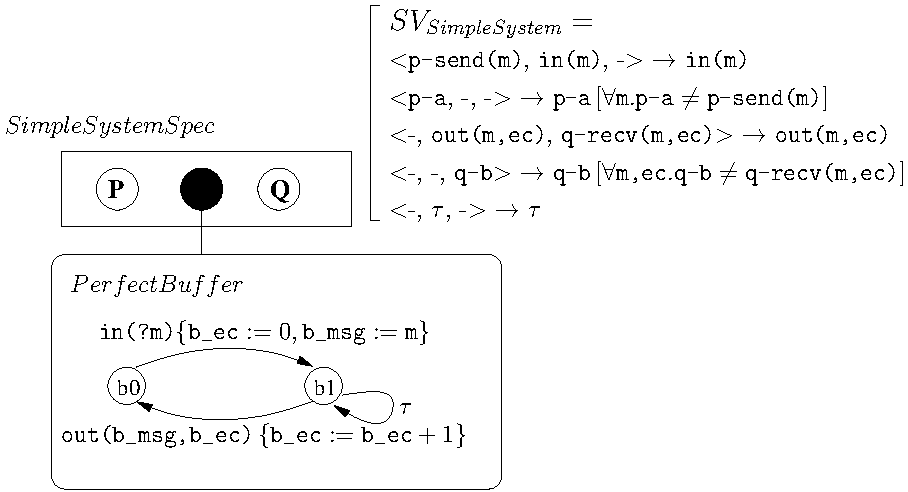
\includegraphics[width=0.7\linewidth]{XFIG/SimpleProt2-Spec.pdf}}
  \caption{pNet of the protocol specification}
   \label{SimpleProtCounter:SpepNet}
\end{figure}

To spare space, we only show and explain here the pNet of the Specification, in Figure \ref{SimpleProtCounter:SpepNet}. In the Specification, the pNet has only one level with two Holes (black box participant processes P and Q) and one pLTS, which describes the external behavior of the (perfect) protocol. 

The actions of P, Q and pLTS (\textit{PerfectBuffer}) are synchronized by synchronization vectors. Process P tries to communicate with Q by action $\texttt{p-send(m)}$ with message data $\texttt{m}$. The protocol gets the message data by action $\texttt{in(m)}$ with assignments $\texttt{b\_ec} \gets 0, \texttt{b\_msg} \gets \texttt{m}$, where $\texttt{b\_ec}$ indicates the number of errors detected and $\texttt{b\_msg}$ represents the message payload.
% Without participants P and Q, the protocol system may failed to send message to P at any situation.
According to the last vector, the Buffer can do $\tau$ actions independently from any P's or Q's moves.
%\TODO{This sentence sounds totally wrong...}
%\Beyond{Corrected.} 
This internal move models the capability of the protocol to detect  errors: $\texttt{b\_ec}$ can increase by one unit at any time by a $\tau$ action. That is also why we can refine this system by its implementation. Finally, the protocol system passes the message and error count by action $\texttt{out(b\_m,b\_ec)}$ and Q receives them by $\texttt{q-recv(b\_m,b\_ec)}$. 
From the second and fourth vectors, P and Q can do any action they want except the meaningful actions ($\texttt{p-send}$ and $\texttt{q-recv}$) of the protocol.
%\TODO{for me, "adding vectors" is not adding constrains, but rather %adding more possible behaviors}
%\Beyond{Corrected.} 



\subsection{Running Example}
% \Beyond{Have a look at this section. I add the missing part back.}\Eric{Yes, it looks good.}

%The running example is a communication protocol via unsafe intermedia (package loss) encoded by OA that allows process P and Q (Hole P and Q) to pass data. This example will help us to illustrate our ideas and algorithms through the entire paper.

%P and Q are black-box participants for the system, and we only care about two actions from each other. Process P can start the communication by action \texttt{p-send(m)} with data \texttt{m} and Process Q can receive the message from the system by action \texttt{q-recv(m,e)} with data \texttt{m} and error count \texttt{ec}. These variables in Hole may replace by certain variables in OA.

\begin{figure}[htbp]
  \centerline{\includegraphics[width=0.7\linewidth]{XFIG/OASpec}}
  \caption{Open Automaton of the protocol Specification  }
   \label{SimpleProtCounter:SpeOA}
\end{figure}

The OA in Figure \ref{SimpleProtCounter:SpeOA}, which is computed from pNet in Figure \ref{SimpleProtCounter:SpepNet}, describes the behaviour of the Specification of the communication protocol. Consider e.g. the Open Transition $\mySS_3$ from state b0 to b1, the Hole P is involved and performs action \texttt{p-send(m)}, its predicate is True, and its Post assigns variables \texttt{b\_ec} and \texttt{b\_msg}, while the resulting action visible here is \texttt{in(m)}.

% \TODO{Why the pictures go to the end of file.}
\begin{figure}[htbp]
    \centerline{\includegraphics[width=0.8\linewidth]{XFIG/OAImpl}}
    \caption{Open Automaton of the Implementation}
    \label{SimpleProtCounter:ImplOA}
\end{figure}

The OA in Figure \ref{SimpleProtCounter:ImplOA} represents the behaviour of the Implementation. In the Implementation, the system becomes more detailed and complex. The states 100, 220, 210, and their actions reflect the internal structure of the protocol. The message data and error counter pass through several variables. We do not need to pay too much attention to its mechanical details, apart from knowing it is just one of all possible implementations.

\begin{figure}[htbp]
   \centerline{\includegraphics[width=0.8\linewidth]{XFIG/WOASpec}}
   \caption{Weak Open Automaton of the Specification %\TODO{change 'formulae' to 'formulas'. And add '(n)' to WOT that have a meta var inside.}\Beyond{Done.}
   }
   \label{SimpleProtCounter:WeakSpecOA}
\end{figure}

\subsubsection{Implementation WOA}

According to Definition \ref{def:buildweakOT}, Weak OAs in Figure \ref{SimpleProtCounter:WeakSpecOA} is built from (strong) OAs from Figure \ref{SimpleProtCounter:SpeOA}; Weak OAs in Figure \ref{SimpleProtCounter:ImplWOA} is built from (strong) OAs from Figure \ref{SimpleProtCounter:ImplOA}. 

According to rule $\WTUn$, each state has a Self-Loop $tau$ transition. 

\begin{mathpar}
W_\tau = \openrule
{\{\}, True, ()}
{s \OTWeakarrow {\tau} s}, \forall s \in \mathcal{S}
\end{mathpar}

Then each OT can be transformed to a WOT by rule $\WTDeux$. For example, we get $\WS_1$, in Figure \ref{SimpleProtCounter:WeakSpecOA}, built from $\mySS_1$, in Figure \ref{SimpleProtCounter:SpeOA}.

\begin{mathpar}
\WS_1 = \openrule
{\{\texttt{P}\mapsto \texttt{p-a}\}, [\forall \texttt{m}. \texttt{p-a} \neq \texttt{p-send(m)} ], ()}
{b0 \OTWeakarrow {\texttt{p-a}} b0}
%, \forall s \in \mathcal{S} \text{(State set of Implementation OA)}
\end{mathpar}

It's the same for $\WS_2$, $\WS_3$, $\WS_5$, $\WS_6$, and all the red arrow lines in Figure \ref{SimpleProtCounter:ImplWOA}.


Rule $\WTTrois$ is the most interesting one. Let us take $\WS_4$ as an example. We have $\mySS_4$ in Figure \ref{SimpleProtCounter:SpeOA}. This OT has the same source state and target state b1 with $\tau$ action. Nevertheless, this OT can occur infinitely, which forms a transition sequence like $\mySS_4^{*}$.

We can build a WOT, $\WS_4(2)$ from the transition sequence $\mySS_4;\mySS_4$ by rule $\WTTrois$:

\begin{mathpar}
\WS_4(2) = \openrule
    {\{\},True,( \texttt{b\_ec } \gets \texttt{b\_ec + 2})}
    {b1 \OTWeakarrow {\tau} b1}
\end{mathpar}

Then we use mathematical induction to get $\WS_4(n)$ from $\mySS_4^{*}$. Here $n$ is a natural number indicating how many times it goes through $\mySS_4$. Actually, $\WS_4(n)$ is a meta weak open transition (meta-WOT), and variable $n$ is a meta-Variable, which will be formalized in the next section (same as $\WS_3(n)$, $\WS_5(n)$, $\WS_6(n)$, $\WS_7(n)$). 
%\Beyond{Maybe we should comment the following sentence.}At that point we will show the WOA of implementation which contains many meta-WOTs.


%\TODO{There used to be an explanation somewhere of your "class of equivalent states \{000,202\}, it seems to have been lost in moving some parts...}
%\Beyond{I added a new paragraph at the end of this section. }
%\Eric{Ok, but I prefer to move it at the beginning.}
%\Beyond{Yes. Accepted.}

\begin{figure}[ht]
   \centerline{\includegraphics[width=0.8\linewidth]{XFIG/WOAImpl}}
   \caption{Weak Open Automaton of the Implementation}
   \label{SimpleProtCounter:ImplWOA}
\end{figure}

%\TODO{We will have to fight against latex floating figures, but only after everything is polished before this point, and definitely fixed} \Beyond{Yes. I like the words "Fight against". It always shows up at somewhere I don't like.}

In Figure \ref{SimpleProtCounter:ImplWOA} , there is a circle covering states 000 and 202, which means these two states are equivalent in some sense. This is because the only transition connecting 000 and 202 is $\WI_{\tau}$, and they all have \textit{similar} self-loop and outgoing transitions. In other words, the environment (observer or other components at the same or higher level of pNet) can not distinguish which state the current system visits.

Let us show some details of the weak transitions in Figure \ref{SimpleProtCounter:ImplWOA}. Most of them are also meta-WOTs. The full set of weak transitions is listed in Appendix \ref{Appendix:Details of Implementation of the Example}.

\medskip
$\WI_{456}(n)$ is constructed from the transition sequence $(\WI_4WT_5\WI_6)^{*}$.
\begin{mathpar}
\WI_{456}(n) = \openrule
         {\{\}, True, 
    (\texttt{s\_ec}\gets \texttt{s\_ec}+n)}
  {100 \OTWeakarrow {\tau} 100}, \forall n \geqslant 0
\end{mathpar}

$\WI_4$ is transformed from $\SI_4$.
\begin{mathpar}
\WI_4= \openrule
         {\{\}, True, 
   (\texttt{m\_msg}\gets \texttt{s\_msg}, \texttt{m\_ec}\gets \texttt{s\_ec}, \texttt{s\_ec}\gets \texttt{s\_ec})}
         {100 \OTWeakarrow {\tau} 210}
\end{mathpar}

$\WI_4(n)$ is constructed by transition sequence $\WI_{456}(n);\WI_4$.
It is easy to see that $\WI_4$ is a particular part of $\WI_4(n)$ when $n = 0$. So, it is enough only to keep $\WI_4(n) $ and omit $\WI_4$.

\begin{mathpar}
\WI_4(n) = \openrule
         {\{\}, True, 
   (\texttt{m\_msg}\gets \texttt{s\_msg}, \texttt{m\_ec}\gets \texttt{s\_ec}+n, \texttt{s\_ec}\gets \texttt{s\_ec}+n)}
         {100 \OTWeakarrow {\tau} 210}, \forall n \geqslant 0
\end{mathpar}


$\WI_3(n)$ is constructed by transition sequence $\WI_{\tau};\WI_3;\WI_{456}(n)$:
\begin{mathpar}
\WI_3(n) = \openrule
  {\{\texttt{P}\mapsto \texttt{p-send(m)}\}, True,
    (\texttt{s\_msg}\gets \texttt{m}, \texttt{s\_ec}\gets n)}
  { \{000,202\} \OTWeakarrow {\texttt{in(m)}} 100}, \forall n \geqslant 0
\end{mathpar}

$\WI_{3a}(n)$ is constructed by transition sequence $\WI_{\tau};\WI_3;\WI_{456}(n);\WI_4$:
\begin{mathpar}
\WI_{3a}(n) = \openrule
  {\{\texttt{P}\mapsto \texttt{p-send(m)}\}, True,
    (\texttt{m\_msg}\gets \texttt{m}, \texttt{m\_ec}\gets n, \texttt{s\_ec}\gets n)}
  { \{000,202\} \OTWeakarrow {\texttt{in(m)}} 210}, \forall n \geqslant 0
\end{mathpar}

For all $\tau$ transitions above, we have a similar WOT that include a non-$\tau$ move from an external action of P or Q, for example:
\begin{mathpar}
\WI_{4P}(n) = \openrule
         {\{\texttt{P}\mapsto \texttt{p-a}\}, [\forall \texttt{m}. \texttt{p-a} \neq \texttt{p-send(m)} ], 
   (\texttt{m\_msg}\gets \texttt{s\_msg}, \texttt{m\_ec}\gets \texttt{s\_ec}+n, \texttt{s\_ec}\gets \texttt{s\_ec}+n)}
         {100 \OTWeakarrow {\texttt{p-a}} 210}
\end{mathpar}

Similarly, we can build all other transitions.






\subsection{Reduce the Running Example}
% \TODO{I don't know how to do it, but these figures are nearly unreadable even on my big screen, you should try to reorganize them...}
% \Beyond{I changed the layout and it's better now.}

Let us apply these three rules for the Implementation OA of our example in Figure \ref{Reduction of Implement OA}A (we don't give fresh names to variables for readability).

\begin{table}[hb]
    \centering
    \caption{Relation Triples for $IOA_2$ and $IOA_1$}
    \begin{tabular}{c c l}
		\hline
	     $IOA_2$ & $IOA_1$ & Predicate\\
	    \hline
        S1 & $000$ & True\\
        S1 & $202$ & True\\
        S4 & $100$ & $\texttt{s\_msg' = s\_msg} \land \texttt{s\_ec' = s\_ec}$\\
        S4 & $210$ & $\texttt{s\_msg' = m\_msg} \land \texttt{s\_ec' = m\_ec}$\\
        S4 & $220$ & $\texttt{s\_msg' = s\_msg} \land \texttt{s\_ec' = s\_ec}$\\
        S4 & $201$ & $\texttt{s\_msg' = r\_msg} \land \texttt{s\_ec' = r\_ec}$\\
	   	\hline
    \end{tabular}
    \label{Table:Relation Triples for IOA2 and IOA1}
\end{table}

We have $ot_{\tau}$ between two pairs of states: $\SI_\tau$ between ($202$,$000$), and $\SI_5$ between ($210$,$220$). The states in each pair have identical Self-Loop transitions. We use $\tau$-Merging in both cases getting new state $S_1$ from state pairs ($000$,$202$) and new state $S_2$ from ($220$,$210$). The rest remains the same. We get the 1st result of minimization, Figure  \ref{Reduction of Implement OA}B.

For $\SI_7$, it is the only outgoing transition from state $S_2$ and ending in state $201$. It matches the conditions for \textit{Forward Merging}. Then we can apply this rule, which merges state $S_2$ and $201$, and returns a new state $S_3$. It is the 2nd result of minimization, Figure  \ref{Reduction of Implement OA}C.

% \TODO{I don't understand the last one, in the forward merging pattern you cannot have a transition from T to S}.
% \Beyond{New conditions and pics of Merging. It can, now.}
% \TODO{Good! So you had to change the proof for the Forward merging in the appendix also...} 
% \Beyond{Yes. Done.}

\begin{table}[hbtp]
    \centering
    \caption{Relation Triples for $IOA_2$ and $\SOA$}
    \begin{tabular}{c c l}
		\hline
	     $IOA_2$ & $\SOA$ & Predicate\\
	    \hline
        S1 & b0 & True\\
        S1 & b0 & True\\
        S4 & b1 & $\texttt{s\_msg' = b\_msg} \land \texttt{s\_ec' = b\_ec}$\\
        S4 & b1 & $\texttt{s\_msg' = b\_msg} \land \texttt{s\_ec' = b\_ec}$\\
        S4 & b1 & $\texttt{s\_msg' = b\_msg} \land \texttt{s\_ec' = b\_ec}$\\
        S4 & b1 & $\texttt{s\_msg' = b\_msg} \land \texttt{s\_ec' = b\_ec}$\\
	   	\hline
    \end{tabular}
    \label{Table:Relation Triples for IOA2 and SOA}
\end{table}

We continue the processing from Figure \ref{Reduction of Implement OA}C. We find that, for $\SI_4$, it is the only transition that comes in $S_3$, apart from Self-Loop transitions. Moreover, the Self-Loop transitions are the same from state $100$ and $S_3$. We can apply rule \textit{Forward Merging} to merge the state pair ($100$,$S_3$), getting a new state $S_4$ and the third result of minimization. Then we cannot find any case that satisfies any one of our reduction rules. It is the final result.

Let us call $IOA_1$ the original Implementation OA, $IOA_2$ it's final reduced OA (Figure \ref{Reduction of Implement OA}D), and $\SOA$ the specification OA.
Even if we have not proven that forward merging preserves Weak FH-Bisimulation, we can check that indeed $IOA_1$ and $IOA_2$ are weak bisimilar, using the TripleSet in table 
\ref{Table:Relation Triples for IOA2 and IOA1}. In these triples, the primed variables are the fresh variables obtained by the successive renamings.
% \Beyond{$SOA$ has a space between S and O. Use \\SOA instead.}\Eric{Good}

%\Beyond{New table:}


\Eric{Moreover, the reduced OA is much easier to compare with the Specification OA from Figure \ref{SimpleProtCounter:SpeOA} because we have now two states matching those of the Specification OA. }
%\Eric{I propose to simplify this:}\Beyond{Let's apply $\sigma_V$ on the final reduced OA. And the variables $s
%\_msg'$ and $s\_ec'$ in Figure \ref{Reduction of Implement OA}D are same as the variables $b\_msg$ and $b\_ec$ in the Specification. 
%}\Eric{as:}

Variables in $s\_msg'$ and $s\_ec'$ in $IOA_2$ correspond to the Specification OA variables $b\_msg$ and $b\_ec$, and we can prove their equivalence using the TripleSets in Table \ref{Table:Relation Triples for IOA2 and SOA}.
% \Beyond{Accepted.}

%\TODO{What about this: \Beyond{The $IOA_2$ and $\SOA$ have Strong FH-Bisimulation relation with TripleSets in Table \ref{Table:Relation Triples for IOA2 and SOA}}.}\Eric{Well, in fact they are not, but we could change small things to make them (like what about 'r\_msg' and 'r\_ec' ?), I'm not sure we have time now. By the way, OT SS7 in Fig 1 is wrong, 'b\_m' should be 'b\_msg' I think}
% \Beyond{Yes. The bug in Spec OA is fixed.}



\begin{figure*}[ht]
	\centering
    \includegraphics[width=\linewidth]{XFIG/ReductionAllInOne}
    \caption{Minimization of the Implementation OA %\TODO{You said you would completely redraw this picture to have larger fonts in the transitions... You simplified the automata B,C,D, but did not really gain in readability. You must change the layout, maybe have only A on the first line, and change the shapes of B,C,D so that they fit in one line ?} 
    %\Beyond{Is it better now?}, \Eric{already better, still too small, try cut lines inside transition elements} \Beyond{New one! I think it's the largest font it could have. Otherwise, it will be ugly.}
    \textbf{(A)} is the original OA, \textbf{(B)} is the 1st result of Reduction, \textbf{(C)} is the 2nd result of Rection, \textbf{(D)} is the 3rd result of Reduction.}
    \label{Reduction of Implement OA}
\end{figure*}


\newpage
\printbibliography

\newpage
\appendix
\section{Details of Implementation of the Example}\label{Appendix:Details of Implementation of the Example} %\TODO{\Beyond{Need checking. I think they are fine.}}

Details of the meta-WOTs is listed here (Figure \ref{SimpleProtCounter:ImplWOA}):

In the first 3 weak transitions, $S$ denotes the set of all global states.

$ W_\tau = \openrule
{\{\}, True, ()}
{S \OTWeakarrow {\tau} S}$

$ \WI_1 = \openrule
{\{\texttt{P}\mapsto \texttt{p-a}\}, [\forall \texttt{m}. \texttt{p-a} \neq \texttt{p-send(m)} ], ()}
{S \OTWeakarrow {\texttt{p-a}} S}$

$ \WI_2 = \openrule
{\{\texttt{Q}\mapsto \texttt{q-b}\}, [\forall \texttt{m,ec}. \texttt{q-b} \neq \texttt{q-recv(m,ec)} ], ()}
{S \OTWeakarrow {\texttt{q-b}} S}$

All following transitions are parametrized by an arbitrary non-negative integer $n\in \mathcal{N}$.


$ \WI_3(n) = \openrule
  {\{\texttt{P}\mapsto \texttt{p-send(m)}\}, True,
    (\texttt{s\_msg}\gets \texttt{m}, \texttt{s\_ec}\gets n)}
  { \{000,202\} \OTWeakarrow {\texttt{in(m)}} 100}
$

$ \WI_{3a}(n) = \openrule
  {\{\texttt{P}\mapsto \texttt{p-send(m)}\}, True,
    (\texttt{m\_msg}\gets \texttt{m}, \texttt{m\_ec}\gets n, \texttt{s\_ec}\gets n)}
  { \{000,202\} \OTWeakarrow {\texttt{in(m)}} 210}
$

$ \WI_{3b}(n) = \openrule
  {\{\texttt{P}\mapsto \texttt{p-send(m)}\}, True,
    (\texttt{s\_ec}\gets n)}
  { \{000,202\} \OTWeakarrow {\texttt{in(m)}} 220}
$

$ \WI_{3c}(n) = \openrule
  {\{\texttt{P}\mapsto \texttt{p-send(m)}\}, True,
    (\texttt{r\_msg}\gets \texttt{m}, \texttt{r\_ec}\gets n)}
  { \{000,202\} \OTWeakarrow {\texttt{in(m)}} 201}
$

$ \WI_4(n) = \openrule
         {\{\}, True, 
   (\texttt{m\_msg}\gets \texttt{s\_msg}, \texttt{m\_ec}\gets \texttt{s\_ec}+n, \texttt{s\_ec}\gets \texttt{s\_ec}+n)}
         {100 \OTWeakarrow {\tau} 210}
$

$ \WI_{4a}(n) = \openrule
         {\{\}, True, 
    (\texttt{s\_ec}\gets \texttt{s\_ec}+n)}
         {100 \OTWeakarrow {\tau} 220}
$

$ \WI_5(n) = \openrule
         {\{\}, True, (\texttt{s\_ec}\gets \texttt{s\_ec}+n)}
         {210 \OTWeakarrow {\tau} 220}
         $

$ \WI_{5a}(n) = \openrule
         {\{\}, True, (\texttt{s\_ec}\gets \texttt{s\_ec}+1+n)}
         {210 \OTWeakarrow {\tau} 100}
         $


$ \WI_6(n) = \openrule
         {\{\}, True, (\texttt{s\_ec}\gets \texttt{s\_ec}+1+n)}
         {220 \OTWeakarrow {\tau} 100}
         $

$ \WI_{6a}(n) = \openrule
         {\{\}, True, 
         (\texttt{m\_msg}\gets \texttt{s\_msg}, \texttt{m\_ec}\gets \texttt{s\_ec}+1+n, \texttt{s\_ec}\gets \texttt{s\_ec}+1+n)}
         {220 \OTWeakarrow {\tau} 210}
         $

% Because 

% $Post_{6a}=\ post_{4}\shortotimes\ post_{456}^*\shortotimes\ post_{6}\\
% = \left( (\texttt{m\_msg}\gets \texttt{s\_msg}, \texttt{m\_ec}\gets \texttt{s\_ec})
% \shortotimes (\texttt{s\_ec}\gets \texttt{s\_ec}+n) \right)
% \shortotimes (\texttt{s\_ec}\gets \texttt{s\_ec}+1) \\
% = (\texttt{m\_msg}\gets \texttt{s\_msg}, \texttt{m\_ec}\gets (\texttt{s\_ec}+1)+n, \texttt{s\_ec}\gets (\texttt{s\_ec}+1)+n)$

\medskip
$ \WI_{456*}(n) = \openrule
         {\{\}, True, 
    (\texttt{s\_ec}\gets \texttt{s\_ec}+n)}
  {100 \OTWeakarrow {\tau} 100}
        $


$ \WI_{564*}(n) = \openrule
         {\{\}, True, 
    (\texttt{m\_msg}\gets \texttt{s\_msg}, \texttt{s\_ec}\gets \texttt{s\_ec}+1+n, \texttt{m\_ec}\gets \texttt{s\_ec}+1+n)}
  {210 \OTWeakarrow {\tau} 210}
        $


$ \WI_{645*}(n) = \openrule
         {\{\}, True, 
    (\texttt{s\_ec}\gets \texttt{s\_ec}+1+n)}
  {220 \OTWeakarrow {\tau} 220}
        $

\medskip
$ \WI_7(n) = \openrule
         {\{\}, True, (\texttt{r\_msg}\gets \texttt{s\_msg}, \texttt{r\_ec}\gets \texttt{s\_ec}+n)}
         {210 \OTWeakarrow {\tau} 201}
         $
         
$ \WI_{7a}(n) = \openrule
         {\{\}, True, (\texttt{r\_msg}\gets \texttt{s\_msg}, \texttt{r\_ec}\gets \texttt{m\_ec}+n+1)}
         {220 \OTWeakarrow {\tau} 201}
         $
         
$ \WI_{7b}(n) = \openrule
         {\{\}, True, (\texttt{r\_msg}\gets \texttt{m\_msg}, \texttt{r\_ec}\gets \texttt{s\_ec}+n)}
         {100 \OTWeakarrow {\tau} 201}
         $
                 
$ \WI_8 = \openrule
         {\{\texttt{Q}\mapsto \texttt{q-recv(r1\_msg,r1\_ec)}\}, True, ()}
         {201 \OTWeakarrow {\texttt{out(r1\_msg,r1\_ec)}} \{202, 000\}}
         $

$ \WI_{8a}(n) = \openrule
         {\{\texttt{Q}\mapsto \texttt{q-recv(m\_msg,m\_ec}+n)\}, True, ()}
         {210 \OTWeakarrow {\texttt{out(m\_msg,m\_ec}+n)} \{202, 000\}}
         $

 $ \WI_{8b}(n) = \openrule
         {\{\texttt{Q}\mapsto \texttt{q-recv(s\_msg,s\_ec}+n+1)\}, True, ()}
         {220 \OTWeakarrow {\texttt{out(s\_msg,m\_ec}+n+1)} \{202, 000\}}
         $

 $ \WI_{8c}(n) = \openrule
         {\{\texttt{Q}\mapsto \texttt{q-recv(s\_msg,s\_ec}+n)\}, True, ()}
         {100 \OTWeakarrow {\texttt{out(s\_msg,s\_ec}+n)} \{202, 000\}}
         $



\medskip
Then for all $\tau$ transitions above we have a similar WOT that include a non-$\tau$ move from an external action of P or Q, like for example:

$ \WI_4P(n) = \openrule
         {\{\texttt{P}\mapsto \texttt{p-a}\}, [\forall \texttt{m}. \texttt{p-a} \neq \texttt{p-send(m)} ], 
   (\texttt{m\_msg}\gets \texttt{s\_msg}, \texttt{m\_ec}\gets \texttt{s\_ec}+n, \texttt{s\_ec}\gets \texttt{s\_ec}+n)}
         {100 \OTWeakarrow {\texttt{p-a}} 210}
$

and

$ \WI_4Q(n) = \openrule
         {\{\texttt{Q}\mapsto \texttt{q-b}\}, [\forall \texttt{m,ec}. \texttt{q-b} \neq \texttt{q-recv(m,ec)} ],
   (\texttt{m\_msg}\gets \texttt{s\_msg}, \texttt{m\_ec}\gets \texttt{s\_ec}+n, \texttt{s\_ec}\gets \texttt{s\_ec}+n)}
         {100 \OTWeakarrow {\texttt{q-b}} 210}
$

but also e.g.:

$ \WI_{456*}P(n) = \openrule
        {\{\texttt{P}\mapsto \texttt{p-a}\}, [\forall \texttt{m}. \texttt{p-a} \neq \texttt{p-send(m)} ], 
    (\texttt{s\_msg}\gets \texttt{s\_msg}, \texttt{s\_ec}\gets \texttt{s\_ec}+n)}
  {100 \OTWeakarrow {\texttt{p-a}} 100}
        $

\bigskip
The following table give a summary of  WOTs, when sharing their names as much as possible.

\begin{table}[ht]
    \centering
    \begin{tabular}{|l|l|c|}
        \hline
        meta-WOT name & Pairs of source states and target states & \# of WOTs \\
        \hline
        $\WI_1$ $\WI_2$ $\WI_\tau$ & $\{(s,s)| s \in \texttt{States of WOA}\} \cup \{(202,000)\} $ & 21 \\
        $\WI_3(n)$ & \{(202,100),(000,100)\} & 2 \\
        $\WI_{3a}(n)$ & \{(202,210),(000,210)\} & 2 \\
        $\WI_{3b}(n)$ & \{(202,220),(000,220)\} & 2 \\
        $\WI_{3c}(n)$ & \{(202,201),(000,201)\} & 2 \\
        $\WI_4(n)$ $\WI_4P(n)$ $\WI_4Q(n)$ & \{(100,210)\} & 3 \\
        $\WI_{4a}(n)$ $\WI_4aP(n)$ $\WI_4aQ(n)$ & \{(100,220)\} & 3 \\
        $\WI_{456*}(n) $ $\WI_{456*}P(n) $ $\WI_{456*}Q(n) $ & \{(100,100)\} & 3 \\
        $\WI_5(n)$ $\WI_5P(n)$ $\WI_5Q(n)$ & \{(210,220)\} & 3 \\
        $\WI_{5a}(n)$ $\WI_{5a}P(n)$ $\WI_{5a}Q(n)$ & \{(210,100)\} & 3 \\
        $\WI_{564*}(n) $ $\WI_{564*}P(n) $ $\WI_{564*}Q(n) $ & \{(210,210)\} & 3 \\
        $\WI_6(n)$ $\WI_6P(n)$ $\WI_6Q(n)$ & \{(220,100)\} & 3 \\
        $\WI_{6a}(n)$ $\WI_{6a}P(n)$ $\WI_{6a}Q(n)$ & \{(220,210)\} & 3 \\
        $\WI_{645*}(n) $ $\WI_{645*}P(n) $ $\WI_{645*}Q(n) $ & \{(220,220)\} & 3 \\
        $\WI_7(n)$ $\WI_7P(n)$ $\WI_7Q(n)$ & \{(210,201)\} & 3 \\
        $\WI_{7a}(n)$ $\WI_{7a}P(n)$ $\WI_{7a}Q(n)$ & \{(220,201)\} & 3 \\
        $\WI_{7b}(n)$ $\WI_{7b}P(n)P$ $\WI_{7b}Q(n)$ & \{(100,201)\} & 3 \\
        $\WI_8(n)$ & \{(201,202),(201,000)\} & 2\\ 
        $\WI_{8a}(n)$ & \{(210,202),(210,000)\} & 2 \\
        $\WI_{8b}(n)$ & \{(220,202),(220,000)\} & 2 \\
        $\WI_{8c}(n)$ & \{(100,202),(100,000)\} & 2 \\
       
        \hline
    \end{tabular}
    \caption{All meta-WOT in the Implementation WOA}
    \label{tab:All WOT in the Implementation WOA}
\end{table}

    \bigskip
    
That makes a total of 73 (meta-)WOTs in the Figure \ref{SimpleProtCounter:ImplWOA}.

\newpage
\subsection{Details of the Bisimulation Checking}\label{Appendix:Details of the Bisimulation Checking}
         
We recall here the relation $\mathcal{R}$ that is the candidate for our meta FH-Bisimulation relation in Table \ref{tab:Bisimulation relation Triples of running example}.

\begin{table}
    \centering
    \begin{tabular}{|c|c|l|}
        \hline
        Spec state & Impl state & Predicate\\
        \hline
        b0 & $000$ & True\\
        b0 & $202$ & True\\
        b1 & $100$ & $\texttt{b\_msg = s\_msg} \land \texttt{b\_ec = s\_ec}$\\
        b1 & $210$ & $\texttt{b\_msg = m\_msg} \land \texttt{b\_ec = m\_ec}$\\
        b1 & $220$ & $\texttt{b\_msg = s\_msg} \land \texttt{b\_ec = s\_ec}$\\
        b1 & $201$ & $\texttt{b\_msg = r\_msg} \land \texttt{b\_ec = r\_ec}$\\
        \hline
    \end{tabular}
    \caption{Bisimulation relation Triples of running example}
    \label{tab:Bisimulation relation Triples of running example}
\end{table}

\bigskip
Considering the first triple <b0, 000, True>, we will prove the following properties, in which $OT<<mWOT$ means that the (strong) open transition $OT$ is covered, in the sense of Definition \ref{def:meta FH-Bisim} by the meta-WOT $mWOT$:

\bigskip
\[\begin{split}
\WS_1 << \WI_1(\emptyset) \qquad \WI_1 << \WS_1(\emptyset) \\
\WS_2 << \WI_2(\emptyset) \qquad \WI_2 << \WS_2(\emptyset) \\
\forall n \geqslant 0, n' \geqslant 0.\WS_3(n) << \WI_3(n') \\
\forall n \geqslant 0, n' \geqslant 0.\WI_3(n) << \WS_3(n')\\
\forall n \geqslant 0, n' \geqslant 0.\WI_3a(n) << \WS_3(n')\\
\forall n \geqslant 0, n' \geqslant 0.\WI_3b(n) << \WS_3(n')\\
\forall n \geqslant 0, n' \geqslant 0.\WI_3c(n) << \WS_3(n')
\end{split}
\]
         
%  Note: if we were using the alternative Weak bisim from Definition \ref{def:Weak-bisim}, we would have a lot more transitions to examine, as we  have 4 weak transitions for $b0$ in the specification weak automaton, but 7 WOTs from 000 in the implementation automaton.
 
 
\clearpage
\section{Examples}
In this section, we introduce some other exciting examples of Weak FH-Bisimulation (meta FH-Bisimulation) for better understanding. By lack of time, we have not yet checked the properties and equivalences of these examples. 

\subsection{Integer Printer}
\label{Integer Printer}
There are two kinds of integer printer, $A(x)$ and $B(y)$, with different structure which can print any positive integer. $A(x)$ and $B(y)$ are strong automata with meta-Variable $x$ and $y$ respectively. 

\begin{figure}[htbp]
	\begin{minipage}[t]{0.49\linewidth}
    \centering   
        \includegraphics[width=\linewidth]{XFIG/mA_x}
        \caption{Integer Printer A(x)}
        \label{A(x) Printer}
	\end{minipage}
	\hspace{0.01\linewidth}
	\begin{minipage}[t]{0.49\linewidth}
    \centering   
        \includegraphics[width=\linewidth]{XFIG/mB_y}
        \caption{Integer Printer B(y)}
        \label{B(y) Printer}    
	\end{minipage}
\end{figure}

And the Predicates in Table \ref{Table:Predicates of A(x) and B(y)}.

\begin{table}[hb]
    \centering
        \begin{tabular}{||c | c | c ||} 
         \hline
         A(x) & B(y) & Predicates  \\
         \hline
         <$a_0$> & <$b_0$> & $a = b = 0$\\
         \hline
         <$a_1$> & <$b_1$> & $odd(a)\land a = b+1$\\
         \hline
         <$a_1$> & <$b_2$> & $a = b$\\
         \hline
         <$a_2$> & <$b_3$> & $True$\\
         \hline
        \end{tabular}
    \caption{Predicates of A(x) and B(y)}
    \label{Table:Predicates of A(x) and B(y)}
\end{table}

It's easy to see that $Amot_0$ and $Bmot_0$ are Similar;
$Amot_2$ and $Bmot_4$ are Similar; $Amot_3$ and $Bmot_5$ are Similar.

We have a meta-WOT set $S = \Big\{mwot_2(y), mwot_{13}(y)\Big\}$ from $B(y)$, where $mwot_2(y)$ is built by $\MWTDeux$ from $Bmot_2(y)$ and $mwot_{13}(y)$ is built by $\MWTTrois$ from meta-OT sequence $Bmot_1(y);Bmot_3$:

%\TODO{to be completed} \Beyond{Done.}
\[
mwot_2(\{y\})= \openrule 
{\{\}, True, (b \gets b + 2y)} { b_0 \OTWeakarrow{\tau} b_2}
\qquad
mwot_{13}(\{y\})= \openrule
{\{\}, True, (b \gets b + 2y + 1)} { b_0 \OTWeakarrow{\tau} b_2}
\]

The proof obligation that $Amot_1(x)$ is covered by $S$ is:
\begin{mathpar}
\forall x \geqslant 0. \Big \{ \Pred_{a_0,b_0} \land True \implies \bigg[ \exists y \geqslant 0. \Big( \tau = \tau \land \Pred_{a_1,b_2}\subst{ [a \gets a + x] \uplus [b \gets b + 2y]} \Big) \\  \lor \Big( \tau = \tau \land \Pred_{a_1,b_2}\subst{ [a \gets a + x] \uplus [b \gets b + 2y + 1]} \Big) \bigg] \Big\}
\end{mathpar}

Instantiated as:

\begin{mathpar}
\forall x \geqslant 0. \Big \{ a=b=0 \implies \big[ \exists y \geqslant 0. ( \tau = \tau \land [a+x=b+2y] )   \lor ( \tau = \tau \land [a+x=b+2y+1] ) \big] \Big\}
\end{mathpar}

That is a tautology.

And $Bmot_1(y)$ and $Bmot_2(y)$ are covered by the meta-WOT built from $Amot_1(y)$.
A interesting part is that $Bmot_3$ is covered by Self-Loop $\tau$ transition built by $\MWTUn$ on state $a_1$. And its proof obligation is:
%\TODO{This is NOT updated, and incorrect. Can you update it, and give explicitly the metaWOT you use for coverage ?}
%\Eric{In fact I think the SelfLoop  you refer should rather be $Amot1;WT1(a_{1\tau})$}
%\Beyond{No. We have $Bmot_3$ starts from $b_1$ to $b_2$. And we have $Pred_{a_1,b_1}$ and $Pred_{a_1,b_2}$. So, the corresponding meta-WOT should start from $a_1$ to $a_1$. So, can't be $Amot1;WT1(a_{1\tau})$.} 
%\Beyond{Update DONE!}

%\TODO{I do not understand your answer...: the formula below is NOT updated: it contains "even(a)" that is no longer in the triples. }
%\Beyond{Well, my bad. I removed them.}

%\TODO{But I hav another problem here, The current def of meta-WOT in the journal version says that "otvars(mwot)" does NOT contain the meta-variables, only the local variables of the transitions... which one is correct ? if otvars() contains the meta variables, I may have to change the proof...}


%\Beyond{I comment my Ambiguous Long Answer. I think, $otvar$ should contain the meta-Variables. What do you think about it? And I should correct all the possible conflicts  in definitions.}
% \Beyond{This a long answer.}

% Several weeks ago, I defined the proof obligation of meta FH-Bisimulation as:\\
% $
% \forall\ otmvars(mwot).\Bigg\{ \Pred_{s,t} \land \Pred_{mwot}\implies
% \displaystyle{\bigvee_{x\in X}\bigg[\exists\ otmvars(mwot_x).
% \Big( \forall j. \gamma_{j}=\gamma_{j x}  \land \Pred_{mwot_x}}\\
% \displaystyle{
%  \land \alpha\!=\!\alpha_x \land  
%  \Pred_{s',t'_x}\subst{\Post_{mwot}\uplus\Post_{mwot_x}}\Big)\bigg]\Bigg\}}
% $

% But, you left a comment "It's OK to write $otvars$ here". So, I changed it back.
% So, I think, the $otvars$ contains the meta-Variables. 

% So, in Definition meta-WOT and meta-WOA, I wrote :

% So now we have three types of variables that can occur in a meta-WOT: OA's variables from $V$ and meta-Variables from $M'$, and local variables of the OT, $otvars(mwot(M'))$.
% \Beyond{Should be: So now we have three types of variables that can occur in a meta-WOT: OA's variables from $V$ and meta-Variables from $M'$, and non-meta-Variables local variables of the OT, $otvars(mwot(M'))$.}

% We denote $otmvars(mwot(M'))=M'$, while $vars$ $(mwot(M'))$ is the set of all variables of the transition, including the automaton variables, $ot$'s local variables, as well as $ot$'s meta variables.

% Then we can redefine $otvars(mwot(M'))=vars$ $(mwot(M'))\backslash otmvars(mwot(M'))$, which will be used in the definition of meta FH-Bisimulation.\\
% ----------------\\
% I commented the last two paragraphs.

% Anyway, I reviewed your proof of Th 3 (I corrected some typos), and understand your question here.

% \Beyond{Over}

\begin{mathpar}
\forall x \geqslant 0. \bigg \{ (odd(a) \land a = b+1 \implies \Big[ \exists y \geqslant 0. \tau = \tau \land [a = b] \subst{b \gets b + 1} \Big] \bigg \}
\end{mathpar}

When $a$ is odd, then the proof obligation can be simplified as:

\begin{mathpar}
\forall x \geqslant 0. \bigg \{ a = b + 1 \implies \Big[ \exists y \geqslant 0.  a = b + 1  \Big] \bigg \}
\end{mathpar}

It's tautology.

When $a$ is even, then the proof obligation can be simplified as:

\begin{mathpar}
\forall x \geqslant 0. \bigg \{ False \implies \Big[ \exists y \geqslant 0.  a = b + 1  \Big] \bigg \}
\end{mathpar}

$False$ implies anything. So, it's tautology. As conclusion, $A(x)$ and $B(y)$ are Alt-meta FH-Bisimulation.

We derive meta-WOT from $A(x)$ as Figure \ref{mwA(x) Printer}.

% \begin{figure}[htbp]
% 	\begin{minipage}[t]{0.49\linewidth}
%     \centering   
%         \includegraphics[width=\linewidth]{XFIG/mwA_x}
%         \caption{Integer Printer A(x) of meta-WOA}
%         \label{mwA(x) Printer}
% 	\end{minipage}
% 	\hspace{0.01\linewidth}
% 	\begin{minipage}[t]{0.49\linewidth}
%     \centering
%         \includegraphics[width=\linewidth]{XFIG/mwA_x}
%         \caption{Integer Printer A(x) of meta-WOA \Beyond{meta-WOA of B(y)....}}
%         \label{mwA(x) Printer}
% 	\end{minipage}
% \end{figure}

\begin{figure}[htbp]
    \centering   
        \includegraphics[width=0.7\linewidth]{XFIG/mwA_x}
        \caption{Integer Printer A(x) of meta-WOA}
        \label{mwA(x) Printer}
\end{figure}

We have $Amwot_i, \forall i \in \{0,1,2,3\}$ come from $Amot_i, \forall i \in \{0,1,2,3\} $ (all the blue lines in Figure \ref{mwA(x) Printer} );
$
Amwot_{\tau} = 
    \openrule 
        {\{\},True,()}
        {s_0 \OTWeakarrow{\tau} s_0}, 
\forall s_0 \in \{a_0,a_1,a_2\}
$;

\begin{minipage}{0.48\linewidth}
    \begin{mathpar}
    Amwot_{10} = 
        \openrule
            {\{\}, True, (a \gets 0)}
            {a_1 \OTWeakarrow{out(a)} a_0} \\
    Amwot_{02}(\{x\}) = 
        \openrule
            {\{\}, True, (a \gets 0 + x)}
            {a_0 \OTWeakarrow{out(a)} a_2} \\
    Amwot_{21}(\{x\}) = 
        \openrule
            {\{\}, True, (a \gets 0 + x)}
            {a_2 \OTWeakarrow{\tau} a_1}
    \end{mathpar}
\end{minipage}
\hfill
\begin{minipage}{0.48\linewidth}
    \begin{mathpar}
    Amwot_{012} = 
        \openrule
            {\{\}, True, (a \gets 0)}
            {a_0 \OTWeakarrow{out(a)} a_0} \\
    Amwot_{120}(\{x\}) = 
        \openrule
            {\{\}, True, (a \gets 0 + x)}
            {a_1 \OTWeakarrow{out(a)} a_1} \\
    Amwot_{201}(\{x\}) = 
        \openrule
            {\{\}, True, (a \gets 0 + x)}
            {a_2 \OTWeakarrow{out(a)} a_2}        
    \end{mathpar}
\end{minipage}

\bigskip
This is a example where the Self-Loop Transition does not introduce a meta-Variable.

\clearpage
\subsection{Coffee Machine}
The idea of coffee vendors comes from paper \cite{BehavioralEquivalences}. It describes how a coffee vending machine works. The differences are that we have Holes, predicates, and assignments, not only action labels. So, with a little extension, we design the new specification open automaton for the vendor machine, in Figure \ref{Specification OA of Coffee Vendors}. It has two states and five actions on them. The vendor machine only has two participants, the customer named Hole P and the manager who cleans the coin box and supplies coffee named Hole M.

Customers can start the transaction, deposit coins, confirm the transaction, and withdraw the extra coins. The manager can manage the machine, supplying new coffee materials. If some customers forget to withdraw, the manager can reset the machine.

\begin{figure}[hb]
\centering   
    \includegraphics[width=\linewidth]{XFIG/CoffeeSpecOA.pdf}
    \caption{Specifications OA of Coffee Vendors}
    \label{Specification OA of Coffee Vendors}
\end{figure}

Then we design the details of the coffee vending machine system in the form of pNet, Figure \ref{pNet Implementation of Coffee Vendors}. It has two levels. The top-level organizes the cooperation of the system and customers. The bottom-level has three leaves automaton, Account, Counter, Money Box, and one Hole M, the manager.

The Account is in charge of the account of current transactions. And it only accepts coins with a face value of 1 Euro and 2 Euro. The price of coffee is 2 Euro. The Counter counts the stock of the countable coffee materials, maybe the capsules. The Money Box records the incomes since the last time the manager clean the coin box. The manager will simultaneously complete the two actions, from the system's view, clean the coin box, and supply the coffee materials (capsules) to the machine's maximum volume ($b_m$ and $m$).

\begin{figure}[htbp]
\centering   
    \includegraphics[width=0.9\linewidth]{XFIG/CoffeepNet.pdf}
    \caption{pNet Implementation of Coffee Vendors}
    \label{pNet Implementation of Coffee Vendors}
\end{figure}

Using the operational semantics of pNets, we get the implementation open automaton from the pNet. In this OA, Figure \ref{Implementations OA of Coffee Vendors}, we have a non-observable action from synchronized vectors, runout. We expect a Weak FH-Bisimulation equivalence between specification and implementation, with the relation Tripleset defined as Table \ref{Table:Bisimulation Relation Triples of Vendor Machine}.

\begin{figure}[htbp]
\centering   
    \includegraphics[width=\linewidth]{XFIG/CoffeeImplOA.pdf}
    \caption{Implementations OA of Coffee Vendors}
    \label{Implementations OA of Coffee Vendors}
\end{figure}

\begin{table}
    \centering
        \begin{tabular}{||c | l | l ||} 
         \hline
         Spec & Impl & Predicates  \\
         \hline\hline
         <b0> & <c0r0a0> & b\_m=m $\land$ b\_coin=coin $\land$ b\_n=n $\land$ b\_a=a\\
         \hline
         <b0> & <c0ra0> & b\_m=m $\land$ b\_coin=coin $\land$ b\_n=n $\land$ b\_a=a\\
         \hline
         <b1> & <c1r1a0> & b\_m=m $\land$ b\_coin=coin $\land$ b\_n=n $\land$ b\_a=a\\
         \hline
         <b1> & <c1r0a0> & b\_m=m $\land$ b\_coin=coin $\land$ b\_n=n $\land$ b\_a=a $\land$ b\_p=2\\
         \hline
        \end{tabular}
    \caption{Bisimulation Relation Triples of Vendor Machine}
    \label{Table:Bisimulation Relation Triples of Vendor Machine}
\end{table}

\newpage
\subsection{Traffic Lights}

% \TODO{Similar work? Reference and Proof.} \Beyond{Finished!}

This example is about traffic lights. Traffic lights are an appropriate use-case for real-time systems \cite{cohen2015systemverilog}. It controls a traffic light at the intersection of a busy highway and a farm road. We simplify it as a normal crossroad and abstract the timer as a Hole in pNet.

There are three kinds of lights in one traffic light, Green, Red, and Yellow. Here, the only participant is a pedestrian who should wait when the Red Light on; walk through the crossroads when Green Light on; Pay attention when the Yellow Light is illuminating. It is just like the specification in Figure \ref{Specification OA of Traffic Light}. Nevertheless, the time interval for each light is set by prior knowledge: 3s for Yellow Light, 17s for Green Light, and 20s for Red Light. With two sets of these traffic light systems controlling two directions, we can control a crossroad.

\begin{figure}[htbp]
\centering   
    \includegraphics[width=0.7\linewidth]{XFIG/TrafficLightSpecOA.png}
    \caption{Specification OA of a Traffic Light}
    \label{Specification OA of Traffic Light}
\end{figure}

Then we design the details of the traffic lights system in the form of pNet, Figure \ref{pNet Implementations of Traffic Light}. It has two levels. On the top level, it describes the cooperation between the traffic light system and pedestrians. 

\begin{figure}[htbp]
\centering   
    \includegraphics[width=0.7\linewidth]{XFIG/TrafficLightpNet.png}
    \caption{pNet Implementations of Traffic Light}
    \label{pNet Implementations of Traffic Light}
\end{figure}

On the bottom level, it describes how the several components, sub-systems, work with each other. The `Light' only control which light should be on, and it will turn on another after turn off the current light; the `Controller' is in charge of communications between the other sub-systems by sending time thresholds and receive data. The `Register' is a counter which starts to count after receiving a time threshold. Furthermore, there is an ideal timer, Hole `T', which has only one action, telling it has just passed 1 second. With the help of the Hole `T', the register can count the seconds correctly.

Using the operational semantics of pNet, we get the implementation open automaton from the pNet. In this OA, Figure \ref{Implementation OA of Traffic Light}, the most interesting part is that the work of register (timer) is independent because the environment cannot observe it. The pedestrian does actions only by the signal of light.

\begin{figure}[htbp]
\centering   
    \includegraphics[width=0.9\linewidth]{XFIG/TrafficLightImpl.png}
    \caption{Implementation OA of Traffic Light}
    \label{Implementation OA of Traffic Light}
\end{figure}

The relation Triples are given like this:

\begin{table}[htbp]
    \centering
        \begin{tabular}{||c | l | l ||} 
         \hline
         Spec & Impl & Predicates  \\
         \hline\hline
         <R> & <RL51> & $c=t \land h=20$\\
         \hline
         <R> & <RL00> & $c=t \land c=h$\\
         \hline
         <G> & <GL11> & $c=t \land h=17$\\
         \hline
         <G> & <GL20> & $c=t \land c=h$\\
         \hline
         <Y> & <YL31> & $c=t \land h=3$\\
         \hline
         <Y> & <YL40> & $c=t \land c=h$\\
         \hline
        \end{tabular}
    \caption{Bisimulation Relation Triples of Traffic Lights}
    \label{Table:Bisimulation Relation Triples of Traffic Lights}
\end{table}

\clearpage

% \section{Minimization and Reduction}
% \label{Appendix:Minimization and Reduction}


% \begin{comment}
% \subsection{One State Minimization}
% \label{Appendix:proof of OSM}
% We start by proving Theorem \ref{theorem:Compress OA in one State} from section \ref{Section:Minimization and Reduction}:

% \textbf{Theorem} \ref{theorem:Compress OA in one State}
%  For any open automaton A, it and OMS(A) are strongly FH-Bisimilar.

% \medskip
% \textit{Proof} Given any open automaton, $A =< J, \mathcal{S}, s_0, V, \T > $, with One State Minimization Definition \ref{def:One State Minimization}, we get a new automaton 
% $OMS(A)= A' =< J, S'=\{ms\}, ms, V\subst{\sigma_V}\cup\{ID\}, \T' > $, that has only one state by construction.

% %\Eric{with my suggestion on Definition \ref{def:One State Minimization}, you get rid of the strange argument about non connected components of the OA (and I'm sure the theorem is true also for OA with non-connected components).
% %So you could write here:\\
% %$A' =< J, S', merged, V\cup\{ID\}, \T' > $, %and by construction you have only one state where $S'=\{merged-state\}$.}

% %\Beyond{You are right. I need to add one more procedure to merge non-connected components. So that, it fits for all OA.}

% %\TODO{Eric: check again this, I think we just don'care about non-connected components}

% %\Beyond{Yes! I need to rewrite all the proof about OMS.}
% %\Beyond{Rewrited!} \Eric{no, rewrite is an irregular verb, you have to write "rewritten" !} \Beyond{Yes, u r right. Remercier.}

% Intuitively, the Strong Bisimulation relation Triples we need is very simple, as follows:
% \begin{table}
%     \centering
%         \begin{tabular}{||c | l | l ||} 
%          \hline
%          Origin Automaton & Minimized Automaton & Predicate  \\
%          \hline\hline
%          <$s_1$> & <$ms$> & $ [\bigwedge_v^{V} v=v' ] \land ID = s_1 $\\
%          \hline
%          <$s_2$> & <$ms$> & $ [\bigwedge_v^{V} v=v' ]\land ID = s_2 $\\
%          \hline
%          <...> & <...> & ...\\
%          \hline
%          <$s_n$> & <$ms$> & $ [\bigwedge_v^{V} v=v' ]\land ID = s_n $\\
%          \hline
%         \end{tabular}
%     \caption{Relation Triples for One State Minimization}
%     \label{Table:Relation Triples for One State Minimization}
% \end{table}

% For any OT in $A$, named $OT_1$:
% \begin{mathpar}
% OT_1=
% \openrule
%  {\set{\beta},\Pred,\Post} 
%  {s_s \OTarrow {\alpha} s_t} \in \T    
% \end{mathpar}

% There exists an corresponding OT from $A'$:
% \begin{mathpar}
% OT_1'=
% \openrule
%  {\set{\beta'},Pred', Post'} 
%  {ms \OTarrow {\alpha\subst{\sigma_V}} ms} \in \T'    
% \end{mathpar}

% According to the Definition \ref{def:One State Minimization}, we have (the $J$ is the set of Hole index):
% \begin{mathpar}
% \forall j \in J.\set{\beta'_j}=\set{\beta_j}\subst{\sigma_V} \\
% Pred' = Pred\subst{\sigma_V} \land [ID = s_s] \\
% Post' = Post\subst{\sigma_V} \cup \{ID \gets s_t\} \\
% \alpha' = \alpha\subst{\sigma_V}
% \end{mathpar}

% We reason the following lemma:

% \begin{lemma}[Predicate of $\sigma_V$ effects]
% \label{lem:Predicate and Substitution}

% Predicates $\bigg [\bigwedge_v^{V} v=v' \bigg]$ just has the same effect like the substitution $\sigma_V$ ($\bigcup_v^{V} \subst{ v\gets v' } $ from Definition \ref{def:Transitions Weak Simulation}) does. Formally, we have:

% \begin{mathpar}
% \bigg [\bigwedge_v^{V} v=v' \bigg ] \implies \set{\beta_j}'^{j \in J} = \set{\beta_j}^{j \in J} ~~;~~
% \bigg [\bigwedge_v^{V} v=v' \bigg ] \implies Pred\subst{\sigma_V} = Pred\\
% \bigg [\bigwedge_v^{V} v=v' \bigg ] \implies Post\subst{\sigma_V} = Post ~~;~~
% \bigg [\bigwedge_v^{V} v=v' \bigg ] \implies \alpha' = \alpha
% \end{mathpar}
% \end{lemma}

% Then we construct the proof obligation of Strong Bisimulation:

% \begin{mathpar}
% \Pred_{s_s,ms} \land \Pred \implies 
% \displaystyle{ \forall j\in J. \set{\beta_j}\!=\!\set{\beta'_{j}} \! \land\! Pred'
%      \!\land\! \alpha\!=\!\alpha'\! \land\!  
%      \Pred_{s_t,ms}\subst{Post \uplus Post'}}
% \end{mathpar}

% With $Pred_{s_s,ms}=\bigg [\bigwedge_v^{V} v=v'  \land ID=s_s \bigg ]$ and $Pred_{s_t,ms}=\bigg [ \bigwedge_v^{V} v=v'  \land ID=s_t \bigg ]$, let's simplify it according to the Lemma \ref{lem:Predicate and Substitution}. Then, we get:

% \begin{mathpar}
% \bigg[ \bigwedge_v^{V} v=v' \land ID=s_s \bigg] \land \Pred \implies 
% \bigg ( \bigg[ \bigwedge_v^{V} v=v' \land ID=s_t \bigg ]\subst{\Post\uplus(\Post \subst{\sigma_V} \uplus \{ID\gets s_t\})} \bigg)
% \end{mathpar}

% $ID$ is new variable, formally $ID \notin V$. So, $ID \notin vars(Post)$ and the final substitution,$\subst{ID \gets s_t}$ , transforms $[ID=s_t]$ into $[s_t=s_t]$. The proof obligation is tautology.

% So, any OT from $s_s$ in $\T$ can be covered by a set of transitions from $ms$ in $\T'$.
% Symmetrically, any OT from $ms$ in $\T'$ can be covered by a set of transitions from $s_s$ in $\T$.

% % \TODO{I think you should explicit the proof obligation for the other direction, it is not the same...}
% % \Beyond{Oui, J'accepte.}

% Formally, the proof obligation goes like :

% \begin{mathpar}
% Pred_{s_s,ms} \land Pred' \implies \forall j \in J. \beta_j = \beta_j 
% \land Pred \land \alpha\!=\!\alpha \land Pred_{s_t,ms}\subst{Post \dotcup Post'}
% \end{mathpar}

% Let us simplify it according to the Lemma \ref{lem:Predicate and Substitution}. Then, we get:

% \begin{mathpar}
% \bigg [ \bigwedge_v^{V} v=v' \land ID=s_s \bigg ] \land \bigg [Pred\subst{\sigma_V} \land ID= s_s \bigg] \implies \\
% Pred \land \bigg( \bigg[\bigwedge_v^{V} v=v' \land ID=s_t \bigg]\subst{Post \uplus (Post\subst{\sigma_V} \cup \{ID \gets s_t\})}\bigg)
% \end{mathpar}

% The final substitution,$\subst{ID \gets s_t}$ , transforms $[ID=s_t]$ into $[s_t=s_t]$. The proof obligation is tautology.

% In summary, $A$ and $OSM(A)$ have strong bisimulation relation using the Tripleset in Table \ref{Table:Relation Triples for One State Minimization}.
% \end{comment}

% \subsection{Local FH-Bisimulation}
% \label{Appendix:Partial FH-Bisimulation}

% We start by formalizing a lemma about local (weak) bisimulation of a subset of open automata. This will allow us to reason locally on the states and transitions affected by reduction rules and prove they preserve the full system's bisimulation.

% Consider that we already have a system described by OA, split into two parts, local and the rest. Now consider another system where only the \emph{`local'} states and transitions are modified w.r.t those of OA, but in a way preserving the structure of states/transitions: we use for that a graph (multi-)morphism $\Phi=(\Phi^S,\Phi^T)$ so that $\Phi^S$ relates the states between the two systems, and $\Phi^T$ relates the transitions coherently, i.e.: if $ot$ is a transition from $s1$ to $s2$, then $\Phi^T(ot)$ is a transition from $\Phi^S(s1)$ to $\Phi^S(s2)$. The following Definition \ref{def:partial FH-Simulation} describes the situation.

% In general, the state mapping of these two systems can be arbitrarily 1 to n and n to 1. In this work, to validate our \emph{Reduction} approach, we only use a special case, where we have only two states in the original local-part and only one state in the reduced local part. In the Reduction, $\Phi^S$ maps two original local states to one combined new state. 

% \begin{definition}[Local FH-Bisimulations]
% \label{def:partial FH-Simulation}

% Let $System= \mylangle J, \mathcal{S}, s_0, V, \T \myrangle$, and split $S$ into a \emph{`local'} subset $LocalS$ and the rest $RS$: $\mathcal{S}=LocalS\uplus RS$.

% Similarly, we split the transitions into 4 sets, local transitions $LocalOT$ are all transitions between states in $LocalS$, including Self-Loops; $incoming$ (resp. $outgoing$) are transitions from $RS$ to $LocalS$ (resp from $LocalS$ to $RS$), and $RT$ transitions between states in $RS$. Let us denote $EffectedT=LocalOT ~\uplus~ incoming ~\uplus~ outgoing$ for short. Then 
% $\T=EffectedT~\uplus~ RT$.

% Consider $System'= \mylangle J, \mathcal{S}', s_0, V, \T' \myrangle$, with:
% $\mathcal{S}'=LocalS'~\uplus~ RS$,
% $\T'=LocalOT'~\uplus~ incoming'$ $\uplus~ outgoing'~\uplus~ RT$, and we have a pair of graph multi-morphisms  
% $\Phi,\Psi$ such that:
% \begin{itemize}
%     \item $\Phi^S$ is a total surjective function on $LocalS$, formally $\forall s \in LocalS. \Phi^S(s) \subset LocalS' \land \forall s' \in LocalS'. \exists s \in LocalS. s' \in \Phi^S(s)$; and the identity (identifying elements as singletons) on the rest of the states in $RS$.
%     \item and symmetrically for $\Psi^S$, with the correspondence condition: $\forall s \in \mathcal{S}, \forall s' \in \Phi^S(s). s \in \Psi^{S'}(s')$.
% \end{itemize} 
% \end{definition}

% \begin{lemma}[Preservation by local bisimulation]
% \label{lem:Preservation by local simulation}
% Let $System$ and $System'$ be Open Auto\-mata obeying Definition \ref{def:partial FH-Simulation}, and $\Phi,\Psi$ their correspondence morphisms. 

% Suppose there exists a Tripleset $\mathcal{R} = <s \in \mathcal{S},s' \in \Phi^S(s), Pred_{s,s'}>$ such that:
% \begin{itemize}
%     \item 
% for each $ot \in EffectedT$, there exists an open transition $ot'$
% with $ot' \in EffectedT'$ and $ot'.sourceState \in \Phi^S(ot.sourceState) \land ot'.targetState \in \Phi^S(ot.targetState)$, and (ot,ot') simulate each other in the sense of Definition \ref{def:Transitions Weak Simulation},
% \item symetrically, for each $ot' \in EffectedT'$, there exist an open transition $ot \in EffectedT$ with $ot.sourceState \in \Psi^S(ot'.sourceState) \land ot.targetState \in \Psi^S(ot'.targetState)$, and (ot,ot') simulate each other,
% \end{itemize}

% then $\mathcal{R}$ is a Weak FH-Bisimulation relation.

% In other terms, the transformation encoded as $\Phi$ preserves weak bisimulation on the whole system.

% \end{lemma}

% \bigskip
% %\textbf{Proof of Lemma \ref{lem:Preservation by local simulation}} 

% \paragraph{Proof sketch:}

% Let $System=<J, \mathcal{S}, s_0, V, \T>$ and $System'=<J, \mathcal{S}', s_0, V, \T'>$
% obeying Definition \ref{def:partial FH-Simulation},
% $WT$ and $WT'$ the sets of weak transitions derived from $T$ and $T'$,
% and TripleSet $\mathcal{R}= <s \in \mathcal{S},s'\in \Phi^S(s), Pred_{s,s'}>$ verifying the hypotheses of Lemma \ref{lem:Preservation by local simulation}.

% According to the Definition of weak bisimulation, we need to prove:

% \begin{itemize}
% \item  For any open transition $OT$ in $\T$:
% $
% OT = \openrule
%     {\beta_j^{j\in J'},\Pred_{OT},\Post_{OT}}
%     {s \OTarrow {\alpha} s'}
% $

% there exists a set of weak open transitions $\symb{WOT}_x^{x\in X}\subseteq \WT $ 
% \begin{mathpar}
% \openrule
%     {\gamma_{j x}^{j\in J_{x}}, \Pred_{OT_x},\Post_{OT_x}}
%     {t \OTWeakarrow {\alpha_x} t'_x}
% \end{mathpar}

% such that $\forall x, \{j\in J'|\beta_j\neq\tau\}=J_{x}, (s',t_x|\Pred_{s',t'_x})\in \mathcal{R}$; 
%  and  \\
 
% $\Pred \land \Pred_{OT} \implies \\
% \hspace{1cm}  \quad \quad
% \displaystyle{\bigvee_{x\in X}\! 
%   \left( \forall j\in J_x. \vis{\beta_j}\!=\!\gamma_{jx}\! \land\! \Pred_{OT_x}
%      \!\land\! \alpha\!=\!\alpha_x\! \land\!  
%      \Pred_{s',t'_x}\subst{\Post_{OT}\uplus\Post_{OT_x}}\right)}$
    
% \item and symmetrically any open transition from $t$ in $\T'$ can be 
%   covered by a set of weak transitions from $s$ in $\WT$.
% \end{itemize}

% Remark that we are in a restrictive case of the general condition for weak FH-Bisimulation: only a small part od system is changed between the 2 systems, and the weak simulation hypothese constrains the transition correspondence to be one to one, rather than one transition "coverd" by a set on the other side.
% So in each case, we search for a pair of open transitions, $(OT, OT')$, that simulate each other. That means there exists a $WOT'_x$ constructed from $OT'$ by rule $\WTDeux$, which fits the previous proof obligation for $OT$.  Meanwhile, there exists a $WOT_x$, which is constructed from $OT$ by rule $\WTDeux$, fits the previous proof obligation for $OT'$ with the same Triples. 
% So, the main proof idea is to prove that for all transition from $System$ there exists one transition from $System'$, keeping the same structure with morphism, that they simulate each other and vise versa. Of course, the Triple sets for the two directions will be the same.

% Let us pick out a state pair ($s1$ and $s2$), from $System$, $s1,s2 \in S$. Then we have Transition set $T_{s1,s2}(\T)$ means these OTs which start from $s1$ and ends in $s2$, formally $\forall s1,s2 \in \mathcal{S}. T_{s1,s2}(\T)=\{ot \in \T| ot~from~s1~to~s2\}$.

% \begin{proof}[Lemma \ref{lem:Preservation by local simulation}]
% \begin{figure}[htbp]
% 	\centering
%     \includegraphics[width=0.8\linewidth]{XFIG/PartialFHBisimulation}
%     \caption{Schema of partial FH-Bisimulation between two systems}
%     \label{fig:partialFHBisimulation}
% \end{figure}

% According to Definition \ref{def:partial FH-Simulation}, the Rest Part of $System$ and $System'$ don't get modified which means they are the same. Then, we can use Fig. \ref{fig:partialFHBisimulation} to show these two systems. $InStateSet \subset LocalS$,
% it contains all states which are the target state of the transitions in $incoming$. $OutStateSet \subset LocalS$,
% it contains all states which are the source state of the transitions in $outgoing$. And it's similar for $InStateSet'$ and $OutStateSet$.

% The proof will be split into 4 parts and 2 directions. Because the 2 directions of simulation are almost the same (especially with the Definition \ref{def:Transitions Weak Simulation}), we only describe one of them, from $System$ to $System'$.

% %part 1
% \bigskip
% \textbf{(1) $\forall s1,s2 \in RS$}
% \medskip

% According to Definition \ref{def:partial FH-Simulation}, binary relation $\Phi$ is a bijection for identity of states in $RS$. And the Rest Part of $System$, $System'$ are same. 
% %when $T_{s1,s2}(\T) \neq \emptyset$
% Then, of course, $\forall t \in T_{s1,s2}(\T)$, $t$ and $\Phi(t)$ are identical, and 
% $(t, \Phi(t))$ simulate each other.

% %part2
% \bigskip
% \textbf{(2) $\forall s1 \in RS \land \forall s2 \in LocalS$}
% \medskip

% When $s1 \in RS/RSOutStateSet \lor s2 \in LocalS/InStateSet$, we have $T_{s1,s2}(\T)=\emptyset$. So, we only care about the case when $s1 \in RSOutStateSet \land s2 \in InStateSet$, meaning $T_{s1,s2}(\T) = incoming$.

% Because of the morphism between $System$ and $System'$, we have:
% \begin{mathpar}
% \bigcup^{s\in InStateSet} \Phi^{S}(s) = InStateSet'
% \qquad and \qquad
% (\bigcup^{s \in S/InStateSet} \Phi^{S}(s)) \cap InStateSet' = \emptyset,\\

% \bigcup^{s\in InStateSet'} \Psi^{S'}(s) = InStateSet
% \qquad  and \qquad
% (\bigcup^{s \in S'/InStateSet'} \Psi^{S'}(s)) \cap InStateSet = \emptyset,\\

% s1' = \Phi^{S}(s1) \land \bigcup ^{s2' \in \Phi^{S}(s2)} T_{s1',s2'}(\T) = incoming' \\
% \end{mathpar}
% So we can conclude that 
% $$\forall ot \in T_{s1,s2}(\T). \forall s2' \in \Phi^{S}(s2). \exists ot' \in T_{s1,s2'}(\T'). s.t. \text{$ot'$ has the same morphism structure as $ot$}$$

% In another word, we can draw $\phi$ out of $\Phi$, which is a binary relation from $InStateSet$ to $InStateSet'$ which use all domain and co-domain. Formally, we use $\phi: InStateSet \to InStateSet'$, where $\phi \subset \Phi$. \TODO{I don't understand why you define $\phi$, you don't use it...}

% According to the hypotheses of Lemma \ref{lem:Preservation by local simulation}, $\forall ot \in EffectedT. \;\exists ot' \in EffectedT'$, $ot$ and $ot'$ simulate each other. 

% Then, we have $\forall ot \in T_{s1,s2}(\T). \exists ot' \in T_{s1',s2'}(\T)$ $ot$ and $ot'$ simulate each other. That means all transitions in $incoming$ get simulated.

% %part3
% \bigskip
% \textbf{(3) $\forall s1 \in LocalS \land \forall s2 \in RS$}
% \medskip

% When $s1 \in LocalS/OutStateSet \lor s2 \in RS/RSInStateSet$, we have $T_{s1,s2}(\T)=\emptyset$. So, we only care about the case that $s1 \in OutStateSet \land s2 \in RSInStateSet$.

% Formally,
% \begin{mathpar}
% \bigcup^{\forall s1 \in RSOutStateSet. \forall s2 \in RSInStateSet} = T_{s1,s2}(\T) = outgoing
% \end{mathpar}

% Because of the morphism between $System$ and $System'$, we have:

% \begin{mathpar}
% \bigcup^{s\in OutStateSet} \Phi^{S}(s) = OutStateSet'\\
% \bigcup^{s\in OutStateSet'} \Psi^{S'}(s) = OutStateSet\\
% (\bigcup^{s \in S/OutStateSet} \Phi^{S}(s)) \cap OutStateSet' = \emptyset\\
% (\bigcup^{s \in S'/OutStateSet'} \Psi^{S'}(s)) \cap OutStateSet = \emptyset\\
% s2' = \Phi^{S}(s2) \land \bigcup ^{s2' \in \Phi^{S}(s2)} T_{s1',s2'}(\T) = outgoing' \\

% \forall ot \in T_{s1,s2}(\T). \forall s1' \in \Phi^{S}(s1). \exists ot' \in T_{s1',s2}(\T'). s.t. ot' \text{has the same morphism structure as} ot.
% \end{mathpar}

% In another word, we can draw $\phi'$ out of $\Phi$, which is a binary relation from $OutStateSet$ to $OutStateSet'$ which use all domain and co-domain. Formally, we use $\phi': OutStateSet \to OutStateSet'$, where $\phi' \subset \Phi$.

% According to Lemma \ref{lem:Preservation by local simulation}, $\forall ot \in EffectedT. \exists ot' \in EffectedT'.$ $ot$ and $ot'$ simulate each other. 

% Then, we have $\forall ot \in T_{s1,s2}(\T). \exists ot' \in T_{s1',s2'}(\T)$ $ot$ and $ot'$ simulate each other. That means all transition in $outgoing$ get simulated.

% %part4
% \bigskip
% \textbf{(4) $\forall s1,s2 \in LocalS$}
% \medskip

% If $T_{s1,s2}(\T) = \emptyset$, according to morphism between $System$ and $System'$,  then $\forall s1' \in \Phi^{S}(s1).\forall s2' \in \Phi^{S}(s2).T_{s1',s2'}(\T) = \emptyset$. 

% So, we only consider the case in which the states' pair contains transition.  

% Formally,
% \begin{mathpar}
% \bigcup^{\forall s1.s2 \in LocalS} T_{s1,s2}(S,T) = LocalOT\\
% \forall s1,s2 \in LocalS.T_{s1,s2}(S,T) \neq \emptyset
% \end{mathpar}

% With the morphism, we have:

% \begin{mathpar}
% \forall s1' \in \Phi^{S}(s1).\forall s2' \in \Phi^{S}(s2).T_{s1',s2'}(\T) \neq \emptyset \\
% \bigcup^{\forall s1' \in \Phi^{S}(s1).\forall s2' \in \Phi^{S}(s2)}T_{s1',s2'}(\T) = LocalOT'\\
% \forall ot \in T_{s1,s2}(\T).\forall s1' \in \Phi^{S}(s1).\forall s2' \in \Phi^{S}(s2). \exists ot' \in T_{s1',s2'}(\T).\\
% s.t. \text{ $ot$ and $ot'$ has the same morphism structure.}
% \end{mathpar}

% Again, according to the hypothesis of Lemma \ref{lem:Preservation by local simulation}, $\forall ot \in EffectedT. \exists ot' \in EffectedT'$, $ot$ and $ot'$ simulate each other.  

% Then, we have $\forall ot \in T_{s1,s2}(\T). \exists ot' \in T_{s1',s2'}(\T)$ $ot$ and $ot'$ simulate each other. That means all transition in $LocalOT$ get simulated.

% So far, we traverse all state pairs, which means we traverse all the transitions. Now, we have the conclusion that $\forall ot \in T, \exists ot' \in T'. s.t.$ $ot$ and $ot'$ simulate each other.

% \TODO{But this is not the end, you still have to show that they fulfill the proof obligation !}

% The other direction of proof is similar to the proof above, which concludes $\forall ot' \in T', \exists ot \in T. s.t.$ $ot$ and $ot'$ simulate each other.

% Then, the transformation encoded as $\Phi$ preserves weak bisimulation.
% \end{proof}

% \subsection{Theorems of Merging}
% \label{Appendix:Theorems of Merging}
% % \TODO{I suggest remove the word "can" here in the definition, and in all occurrences later. It's better to write "A and B simulate each other"}
% % \Beyond{Yes. Accepted.}

% \subsubsection{Tau Merging}
% \label{Appendix:Proof on tau Merging}
% % \TODO{Any reviewer reading a proof starting by "it's easy to see that" (especially if he/she has not fully memorized all your previous huge formulas, not to mention Rule WT2!) will be very upset. What makes this proof "easy", is that this particular Weak Bisimulation analysis is much simpler than the general case, because transitions correspond one to one, and the transitions themselves are mostly unchanged, so you don't need to go through detailed proof conditions on predicates and posts. But you cannot assume the reviewer will understand this by himself, you have to write it in some sufficiently formal way. I would start, at least, by giving a formal def of your "simulate each other" property. Then explain shortly why it applies easily to all pairs in the next paragraph.}

% % \Beyond{Yes. I will make it more sufficient.}

% Using the notion of \textit{Similar} in section \ref{section:Transition Merging Principles}, and the pre-conditions of $\tau$ Merging `Self-Loop transitions in $S$ and $T$ are Similar Self-Loop transitions, or $S$ and $T$ do not have Self-Loop transitions.', it is easy to see that transition in $I$ is \textit{Similar} with the transition in J (I and J can be empty set).

% The procedure of $\tau$ Merging only changes the source state and target state of transitions. So with $\bigwedge_v^{V} v=copy(v)$ in Triples, $Sin_i^{i \in I'}$ and corresponding $STin_i^{i \in I'}$ simulate each other; $Sslt_i^{i \in I}$ and corresponding $STslt_k^{k \in K}$ simulate each other;  $Tslt_i^{i \in I}$ and corresponding $STslt_k^{k \in K}$ simulate each other; $Tout_i^{i \in I'}$ and corresponding $STout_i^{i \in I'}$ simulate each other; $Tout_j^{j\in ''}$ and corresponding $STslt_j^{j \in J''}$ simulate each other.


% \begin{figure}[htbp]
% 	\begin{minipage}[t]{0.55\linewidth}
% 		\centering
%         \includegraphics[width=\linewidth]{XFIG/BeforeTauMerging.pdf}
%         \caption{Before tau Merging}
%         \label{Figure:Before tau Merging for proof}
% 	\end{minipage}
% 	\begin{minipage}[t]{0.4\linewidth}
% 		\centering
%         \includegraphics[width=\linewidth]{XFIG/AfterTauMerging.pdf}
%         \caption{After tau Merging}
%         \label{Figure:After tau Merging for proof}
% 	\end{minipage}
% \end{figure}

% \textbf{$OT\tau$ can be simulated:}
% The only thing left is that we need to find a WOT from result OA that simulates the transition $OT\tau$. It can be simulated by $tau$ transition built from rule $\WTDeux$ in the result OA.

% In $OT_\tau$, we have $\set{\beta} = \emptyset$, $\Pred = True$, $Post = \emptyset$ and $\alpha$ is a non-observable action.

% So, the proof obligation is:

% \medskip
% $
% \Pred_{s,st} \land True \!\implies\! \beta = \{\} \land True \land \underline{\alpha} = \tau \land Pred_{t,st}
% $
% \medskip

% With Triple Predicates $\Pred_{s,st} = \Pred_{t,st}$, the proof obligation is tautology.

% So, these two parts have weak bisimulation relations.


% \subsubsection{Forward Merging}
% \label{Appendix:Proof on Forward Merging}

% Just like the previous mention about $\tau$ Merging, with 
% $\bigg [\bigwedge_v^{V} v=v' \bigg]$, we know that $Sin_i^{i \in I'}$ and corresponding $STin_i^{i \in I'}$ simulate each other; $Sslt_i^{i \in I}$ and corresponding $STslt_k^{k \in K}$ simulate each other; transition in $I$ is Similar with transition in J; $Tslt_i^{i \in I}$ and corresponding $STslt_k^{k \in K}$ simulate each other; $Sout_i^{i \in I''}$ and corresponding $STout_i^{i \in I''}$ simulate each other.

% \begin{figure}[htbp]
% 	\begin{minipage}[t]{0.49\linewidth}
% 		\centering
%         \includegraphics[width=\linewidth]{XFIG/BeforeForwardMerging.pdf}
%         \caption{Before Forward Merging}
%         \label{Figure:Before Forward Merging for proof}
% 	\end{minipage}
% 	\begin{minipage}[t]{0.49\linewidth}
% 		\centering
%         \includegraphics[width=\linewidth]{XFIG/AfterForwardMerging.pdf}
%         \caption{After Forward Merging}
%         \label{Figure:After Forward Merging for proof}
% 	\end{minipage}
% \end{figure}

% This leaves us with 5 non-trivial correspondences to establish, namely
% that $STout_j^{j \in J'}$, $STslt_j^{j \in J''}$ in the result OA can be simulated; $OT$, $Tout_j^{j\in J'}$ and $Tout_j^{j \in J''}$ in original OA can be simulated.
 
% \bigskip\noindent
% \textbf{(1) $STout_j^{j \in J'}$ can be simulated:}
% \medskip

% Then we need to prove $STout_j^{j \in J'}$ can be simulated by a WOT, which is built from transition sequence $OT-Tout_j^{j \in J'}$. $s'$ refers to two states; one is in the original OA, which is the target state of $Tout_j^{j \in J'}$; the other is in the result OA, which is the target state of $STout_j^{j \in J'}$.
% \smallskip
% Let $WOT_j$ be the result of \textit{Forward Merging} with OT and $Tout_j$, then the proof obligation is:

% \medskip
% $\Pred_{s,st} \land STout_j.Pred \!\implies\! \\
% STout_j.\beta = WOT_j.\beta \land WOT_j.Pred \land WOT_j.Action = STout_j.Action \land Pred_{s',s'}\subst{WOT_j.Post \uplus STout_j.Post}
% $
% \medskip

% According to merging rules $\MTUn$ and construction rule $\WTTrois$, we know their Hole actions, transition actions, and predicates should be the same.

% So, the proof obligation simplifies as:

% \medskip
% $\Pred_{s,st}  \!\implies\! \Pred_{s',s'}\subst{ (Tout_j^{j \in J} \shortotimes OT.Post ) \uplus ( Tout_j^{j \in J} \shortotimes OT.Post ) }
% $
% \medskip

% With predicates $\Pred_{s,st} = \Pred_{s',s'}$ , the proof obligation is tautology.

% \bigskip\noindent
% \textbf{(2) $STslt_j^{j \in J''}$ can be simulated:}
% \medskip

% $STslt_j^{j \in J''}$ is the result of applying rule $\MTUn$ on $OT$ and transition $Tout_j^{j\in J''}$. 


% \begin{minipage}[h]{0.48\linewidth}
%     \centering
%     \begin{mathpar}
%         OT = 
%         \openrule
%          {\set{\gamma}, Pred, Post} 
%          {S \OTarrow{\underline {\alpha}} T}
%      \end{mathpar}
% \end{minipage}
% \hfill
% \begin{minipage}[h]{0.48\linewidth}
%     \centering
%     \begin{mathpar}
%         Tout_j^{j \in J''} = 
%         \openrule
%          {\set{\gamma_1}, Pred_1, Post_1} 
%          {T \OTarrow{\alpha_1} S}
%     \end{mathpar}
% \end{minipage}

% \bigskip

% After applying $\MTUn$ on $OT$ and $Tout_j^{j \in J''}$, merging state $S$,$T$, applying $\sigma_V$, we get $STslt_j^{j \in J''}$ as :

% \begin{mathpar}
% \centering
%     STslt_j^{j \in J''} = 
%     \openrule
%      {(\set{\gamma}\dotcup \set{\gamma_1}\subst{\Post})\subst{\sigma_V}, 
%      (Pred \land Pred_1\subst{Post})\subst{\sigma_V}, 
%      (Post_1\shortotimes Post)\subst{\sigma_V}} 
%      {ST \OTarrow {(\alpha_1\subst{Post})\subst{\sigma_V}}\ ST}
% \end{mathpar}

% After applying $\WTTrois$ to construct a WOT from $OT$ and $Tout_j^{j \in J''}$, we get $WOT_j^{j \in J''}$:

% \begin{mathpar}
% \centering
%     WOT_j^{j \in J''} = 
%     \openrule
%      {\set{\gamma}\dotcup \set{\gamma_1}\subst{\Post}, 
%      Pred \land Pred_1\subst{Post}, 
%      Post_1\shortotimes Post} 
%      {S \OTWeakarrow{\alpha_1\subst{Post}}\ S}
% \end{mathpar}

% With predicate $\Pred_{S,ST} = \bigg [ \bigwedge_v^{V} v=v' \bigg ]$ and Lemma \ref{lem:Predicate and Substitution} , it's easy to see that the proof obligation about $STslt_j^{j \in J''}$ being simulated by $WOT_j$ is a tautology.

% \bigskip\noindent
% \textbf{(3) $Tout_j^{j \in J''}$ can be simulated:}
% \medskip

% The previous context continues. 
% A WOT which is constructed from $STslt_j^{j \in J''}$:

% \begin{mathpar}
% \centering
%     WOT_{STslt_j} = 
%     \openrule
%      {(\set{\gamma}\dotcup \set{\gamma_1}\subst{\Post})\subst{\sigma_V}, 
%      (Pred \land Pred_1\subst{Post})\subst{\sigma_V}, 
%      (Post_1\shortotimes Post)\subst{\sigma_V}} 
%      {S \OTWeakarrow {(\alpha_1\subst{Post})\subst{\sigma_V}}\ S}
% \end{mathpar}

% The proof obligation that $Tout_j^{j \in J''}$ be simulated by $WOT_{STslt_j}$:

% \bigskip
% $
% Pred_{T,ST} \land Pred_1 \implies \\
% \quad \quad  \forall j \in J. \set{\gamma_1}_j = (\set{\gamma}\dotcup \set{\gamma_1}\subst{\Post})_j\subst{\sigma_V} 
% \land \alpha_1 = (\alpha_1\subst{Post})\subst{\sigma_V} 
% \land (Pred \land Pred_1\subst{Post})\subst{\sigma_V} 
% \land Pred_{S,ST}\subst{Post \uplus (Post_1\shortotimes Post)\subst{\sigma_V}}
% $

% \bigskip
% Here, the $J$ is the set of the Hole index.
% We have $Pred_{T,ST}=\bigg [ [\bigwedge_v^{V} v=v'] \land [\bigwedge^{i \in K} [v_i = e_i]~where~ \subst{v_i \gets e_i} \in Post ] \bigg ]$.

% $\bigg [\bigwedge^{i \in K} [v_i = e_i]~where~ \subst{v_i \gets e_i} \in Post \bigg]$ just "Simulate" the effect of the substitution $Post$. So, we have:

% \medskip
% $
% \bigwedge^{i \in K} [v_i = e_i]~where~ \subst{v_i \gets e_i} \in Post \implies \alpha_1 = \alpha_1\subst{Post}
% $

% \bigskip

% And with Lemma \ref{lem:Predicate and Substitution}, we have:\
% $[\bigwedge_v^{V} v=v'] \implies \alpha_1 = (\alpha_1\subst{Post})\subst{\sigma_V}$
% \medskip

% It's the same for $Pred$ and $Post$.

% \bigskip
% Then, we have:
% $Pred_{S,ST}\subst{Post \uplus (Post_1\shortotimes Post)\subst{\sigma_V}}=[\bigwedge_v^{V} v=v']\subst{Post \uplus (Post_1\shortotimes Post)\subst{\sigma_V}}=True$
% \medskip

% With condition $\forall~holeAction \in \set{\beta} = \tau~or~empty$, we have:

% \begin{mathpar}
% \forall j \in J. \set{\gamma_1}_j = (\set{\gamma}\dotcup \set{\gamma_1}\subst{\Post})_j\subst{\sigma_V}
% \end{mathpar}

% After simplifying the proof obligation, we only need to prove:

% \begin{mathpar}
% Pred_{T,ST} \land Pred_1 \implies Pred
% \end{mathpar}

% From the pattern, we know $OT$ is the only transition that comes in $T$ (besides the Self-Loop transitions), and $Tout_j^{j\in J''}$ goes out $T$. That means only and only if the $Pred$ is $True$, then the transition flow goes through $OT$ and $Tout_j^{j\in J''}$ ($Pred_j$ also should be $True$). In other words, when we are talking about which $WOT$ can simulate $Tout_j^{j\in J''}$, the subtext is "$Pred$ is $True$". Otherwise, $Tout_j^{j\in J''}$ will never happen, and it is meaningless to simulate an open transition that would never happen.

% However, it is necessary to talk about the meaningless case, $Pred=False$. It means the $OT$ will never happen. All transitions start from $T$, these states are only available from $T$, and their transitions will never happen or be reached. In that case, the guard of $STslt_j$, $Pred\land\Pred_1\subst{Post}$, is $False$ which means $STslt_j^{j \in J''}$ will never happen. Of course, $STout_j^{j \in J'}$ will never happen. So, the reduction would not increase any possibility that the original OA does not have.

% In summary, $Tout_j^{j \in J''}$ can be simulated.

% \bigskip\noindent
% \textbf{(4) $OT$ can be simulated:}
% \medskip

% $OT$ can be simulated by a $tau$ transition built from rule $\WTDeux$. In OT, we have $\set{\beta} = \{\}$, $\Pred = True$, $Post = ()$ and $\alpha$ is a non-observable action.

% The proof obligation is:

% \medskip
% $\Pred_{s,st} \land OT.\Pred \!\implies\! \beta = \{\} \land True \land \alpha = \tau \land Pred_{t,st}\subst{OT.Post}$
% \medskip

% We have $\Pred_{t,st} =Pred_{T,ST}=\bigg [ [\bigwedge_v^{V} v=v'] \land [\bigwedge^{i \in K} [v_i = e_i]~where~ \subst{v_i \gets e_i} \in Post ] \bigg ]$

% \bigskip
% then, 
% $Pred_{t,st}\subst{OT.Post} = [ v_i = e_i]^{i \in K} \subst{v_i \gets e_i}^{i \in K} = \{ e_i = e_i\}^{i \in K}$.
% \smallskip

% With predicate $\Pred_{s,st} = [\bigwedge_v^{V} v=v']$, the simplified proof obligation should be:

% \medskip
% $OT.\Pred \!\implies\! True$
% \medskip

% The proof obligation is tautology.

% \bigskip\noindent
% \textbf{(5) $Tout_j^{j\in J'}$ can be simulated:}
% \medskip

% $Tout_j^{j\in J'}$ can be simulated by WOT from corresponding $STout_j^{j \in J'}$

% The proof obligation is:

% \medskip
% $\Pred_{t,st} \land Tout_j.\Pred \!\implies\! \\ Tout_j.\beta = STout_j.\beta \land STout_j.Pred \land Tout_j.Action = STout_j.Action \land Pred_{s',s'}\subst{Tout_j.Post \uplus STout_j.Post}$
% \medskip

% According to merging rule $\MTUn$, after merging states and applying substitution $\sigma_V$, the proof obligation becomes:

% \medskip
% $[ v_i = e_i ]^{i \in I} \land Tout_j.\Pred 
% \!\implies\!  \\
% Tout_j.\beta = (Tout_j.\beta\subst{OT.Post})\subst{\sigma_V} 
% \land (Tout_j.Pred\subst{OT.Post} \land OT.Pred )\subst{\sigma_V}
% \land Tout_j.Action = (Tout_j.Action\subst{OT.Post} )\subst{\sigma_V}
% \land \\ Pred_{s',s'}\subst{Tout_j.Post \uplus (Tout_j.Post\subst{OT.Post})\subst{\sigma_V}}$
% \medskip

% Just like the proof in \textbf{(3)}, we have:

% \medskip
% $[ v_i = e_i ]^{i \in K} \land Tout_j.\Pred \!\implies\! \\
% Tout_j.\beta = (Tout_j.\beta\subst{OT.Post})\subst{\sigma_V} 
% \land (Tout_j.Pred\subst{OT.Post})\subst{\sigma_V}  
% \land Tout_j.Action = (Tout_j.Action\subst{OT.Post})\subst{\sigma_V}$

% \medskip
% $Pred_{s',s'}\subst{Tout_j.Post \uplus (Tout_j.Post\subst{OT.Post})\subst{\sigma_V}} = True$
% \bigskip

% After simplifying the proof obligation, we only need to prove:

% \medskip
% $[ v_i = e_i ]^{i \in K} \land Tout_j.\Pred \!\implies\! 
% OT.Pred$
% \medskip

% Just like discussion in \textbf{(3)}, if $OT.Pred=False$, then $Tout_j^{j \in J'}$ would never happen, which is meaningless. When $OT.Pred=True$, the proof obligation is tautology.

% This terminates the proof for \textit{Forward Merging}.

% \subsubsection{Backward Merging}
% \label{Appendix:Proof on Backward Merging}

% The proof is similar to the previous sub-section.

\end{document}
